% ============================================================
% BÁO CÁO MÔN HỌC: HỆ THỐNG KHUYẾN NGHỊ
% CHỦ ĐỀ 9: SESSION-BASED RECOMMENDATION SYSTEM
% Trường Đại học Công nghiệp TP.HCM - Khoa CNTT
% ============================================================
\documentclass[12pt, a4paper]{article}

% === Ngôn ngữ và font ===
\usepackage[utf8]{inputenc}
\usepackage[vietnamese]{babel}
\usepackage[T5]{fontenc}

% === Trang và bố cục ===
\usepackage[left=2.5cm, right=2.5cm, top=2.5cm, bottom=2.5cm]{geometry}
\usepackage{setspace}
\onehalfspacing

% === Toán học ===
\usepackage{amsmath, amssymb, amsfonts}

% === Bảng ===
\usepackage{booktabs}
\usepackage{multirow}
\usepackage{array}
\usepackage{longtable}
\usepackage{tabularx}
\newcolumntype{L}[1]{>{\raggedright\arraybackslash}p{#1}}

% === Hình ảnh ===
\usepackage{graphicx}
\graphicspath{{../output/}{./}}
\usepackage{float}
\usepackage{subcaption}

% === Thuật toán ===
\usepackage[ruled, vlined, linesnumbered]{algorithm2e}
\SetAlgorithmName{Thuật toán}{Thuật toán}{Danh sách thuật toán}

% === Code ===
\usepackage{listings}
\usepackage{xcolor}
\lstset{
    language=Python,
    basicstyle=\ttfamily\small,
    keywordstyle=\color{blue}\bfseries,
    commentstyle=\color{gray}\itshape,
    stringstyle=\color{red!70!black},
    numberstyle=\tiny\color{gray},
    numbers=left,
    numbersep=5pt,
    breaklines=true,
    frame=single,
    backgroundcolor=\color{gray!5},
    showstringspaces=false,
    tabsize=4,
    captionpos=b,
    xleftmargin=1cm,
    framexleftmargin=0.5cm,
}

% === Hyperlink ===
\usepackage{hyperref}
\hypersetup{
    colorlinks=true,
    linkcolor=blue!70!black,
    citecolor=green!50!black,
    urlcolor=blue!60!black,
}

% === Tiêu đề và mục lục ===
\usepackage{titlesec}
\titleformat{\section}{\Large\bfseries}{\thesection.}{0.5em}{}
\titleformat{\subsection}{\large\bfseries}{\thesubsection.}{0.5em}{}
\titleformat{\subsubsection}{\normalsize\bfseries}{\thesubsubsection.}{0.5em}{}

% === Đánh số hình, bảng theo section ===
\usepackage{chngcntr}
\counterwithin{figure}{section}
\counterwithin{table}{section}
\counterwithin{equation}{section}

% === Header/Footer ===
\usepackage{fancyhdr}
\pagestyle{fancy}
\fancyhf{}
\fancyhead[L]{\small\leftmark}
\fancyhead[R]{\small Chủ đề 9: Session-based RS}
\fancyfoot[C]{\thepage}
\renewcommand{\headrulewidth}{0.4pt}
\setlength{\headheight}{17pt}

% === Indent đoạn văn ===
\usepackage{indentfirst}
\setlength{\parindent}{1cm}

% === Gói bổ sung ===
\usepackage{enumitem}
\usepackage{caption}
\usepackage{url}

% ============================================================
\begin{document}
\hypersetup{pageanchor=false}

% ============================================================
% TRANG BÌA
% ============================================================
\begin{titlepage}
\begin{center}

\textbf{\normalsize BỘ CÔNG THƯƠNG}\\[0.15cm]
\textbf{\normalsize TRƯỜNG ĐẠI HỌC CÔNG NGHIỆP TP. HỒ CHÍ MINH}\\[0.15cm]
\textbf{\normalsize KHOA CÔNG NGHỆ THÔNG TIN}\\[0.45cm]

\begin{figure}[H]
\centering

\includegraphics[width=4cm]{logo.png}
\end{figure}

\vspace{1cm}

{\LARGE\bfseries BÁO CÁO MÔN HỌC}\\[0.5cm]
{\Large\bfseries HỆ THỐNG KHUYẾN NGHỊ}\\[0.3cm]
{\Large (Recommender Systems)}\\[1.5cm]

\rule{12cm}{0.5pt}\\[0.5cm]
{\Huge\bfseries Chủ Đề 9}\\[0.3cm]
{\LARGE\bfseries HỆ THỐNG KHUYẾN NGHỊ\\DỰA TRÊN PHIÊN DUYỆT WEB}\\[0.3cm]
{\Large (Session-based Recommendation System)}\\[0.5cm]
\rule{12cm}{0.5pt}

\vspace{2cm}

\begin{tabular}{@{}l L{9.2cm}@{}}
\textbf{Giảng viên hướng dẫn:} & TS. Lê Thị Vĩnh Thanh \\[0.3cm]
\textbf{Chủ đề thực hiện:} & Chủ đề 9 \\[0.3cm]
\textbf{Thành viên:} & 1. Phan Nguyễn Mai Phương -- MSHV: 25002711 \\
                     & 2. Ngô Quốc Hoàng -- MSHV: 25001771 \\
                     & 3. Bùi Thức Nam -- MSHV: 25003881 \\
\end{tabular}

\vfill

{\large TP. Hồ Chí Minh, \today}

\end{center}
\end{titlepage}
\hypersetup{pageanchor=true}
\pagenumbering{roman}

% ============================================================
% DANH MỤC TỪ VIẾT TẮT
% ============================================================
\newpage
\phantomsection
\addcontentsline{toc}{section}{DANH MỤC TỪ VIẾT TẮT}
\section*{DANH MỤC TỪ VIẾT TẮT}

\begin{longtable}{@{}p{2.8cm} p{12.5cm}@{}}
\toprule
\textbf{Viết tắt} & \textbf{Diễn giải} \\
\midrule
\endfirsthead
\toprule
\textbf{Viết tắt} & \textbf{Diễn giải} \\
\midrule
\endhead
\bottomrule
\endfoot

RS       & Recommendation System -- Hệ thống khuyến nghị \\
CF       & Collaborative Filtering -- Lọc cộng tác \\
SBR      & Session-Based Recommendation -- Khuyến nghị dựa trên phiên \\
KNN      & K-Nearest Neighbors -- K láng giềng gần nhất \\
SKNN     & Session-based K-Nearest Neighbors -- KNN trên phiên \\
RNN      & Recurrent Neural Network -- Mạng nơ-ron hồi quy \\
GRU      & Gated Recurrent Unit -- Đơn vị hồi quy có cổng \\
GRU4Rec  & Mô hình khuyến nghị dùng GRU (Hidasi et al., ICLR 2016) \\
LSTM     & Long Short-Term Memory -- Bộ nhớ dài-ngắn hạn \\
BPTT     & Backpropagation Through Time -- Lan truyền ngược theo thời gian \\
BPR      & Bayesian Personalized Ranking -- Hàm mất mát xếp hạng cá nhân hoá \\
Adam     & Adaptive Moment Estimation -- Thuật toán tối ưu Adam \\
MRR      & Mean Reciprocal Rank -- Trung bình nghịch đảo hạng \\
NDCG     & Normalized Discounted Cumulative Gain -- Lợi ích tích luỹ chuẩn hoá \\
Recall@K & Tỉ lệ phiên có item đúng nằm trong Top-K gợi ý \\
NLP      & Natural Language Processing -- Xử lý ngôn ngữ tự nhiên \\
ICLR     & International Conference on Learning Representations \\
CIKM     & Conference on Information and Knowledge Management \\
RecSys   & ACM Conference on Recommender Systems \\
UMUAI    & User Modeling and User-Adapted Interaction (tạp chí) \\

\end{longtable}

% ============================================================
% BẢNG THUẬT NGỮ
% ============================================================
\newpage
\phantomsection
\addcontentsline{toc}{section}{BẢNG THUẬT NGỮ}
\section*{BẢNG THUẬT NGỮ}

\begin{longtable}{@{}p{4.2cm} p{11cm}@{}}
\toprule
\textbf{Thuật ngữ} & \textbf{Định nghĩa} \\
\midrule
\endfirsthead
\toprule
\textbf{Thuật ngữ} & \textbf{Định nghĩa} \\
\midrule
\endhead
\bottomrule
\endfoot

Session (phiên)          & Một chuỗi tương tác liên tiếp của một người dùng trên website trong khoảng thời gian ngắn, ví dụ chuỗi click sản phẩm trong cùng lần truy cập. \\
Item                     & Đối tượng được khuyến nghị (sản phẩm, tin tức, video, …); mỗi item có một mã định danh duy nhất. \\
Click                    & Một hành động tương tác của người dùng với một item trong phiên. \\
Người dùng ẩn danh       & Người dùng không đăng nhập, không có ID cố định; chỉ nhận diện được trong phạm vi phiên hiện tại. \\
Cold-start               & Tình huống thiếu dữ liệu lịch sử (user mới, item mới, phiên mới) khiến mô hình truyền thống khó dự đoán. \\
Embedding                & Vector số thực biểu diễn item trong không gian ẩn; các item tương đồng có embedding gần nhau. \\
Hidden state             & Trạng thái ẩn của mạng hồi quy, tóm tắt thông tin chuỗi click đã quan sát đến thời điểm hiện tại. \\
Top-N recommendation     & Danh sách $N$ item có điểm số cao nhất do mô hình sinh ra. \\
Inverted index           & Cấu trúc dữ liệu ánh xạ mỗi item về tập phiên chứa item đó; dùng để tăng tốc tính tương đồng phiên trong SKNN. \\
Hyperparameter           & Tham số do người thiết kế chọn trước khi huấn luyện (ví dụ $K$, learning rate, kích thước embedding), không học từ dữ liệu. \\
Epoch                    & Một lượt mô hình quét qua toàn bộ tập huấn luyện. \\
Mini-batch               & Tập con nhỏ các mẫu được tính gradient cùng lúc trong một bước cập nhật. \\
Train/Test split         & Việc chia dữ liệu thành tập huấn luyện và tập kiểm tra; trong báo cáo này chia theo trục thời gian. \\
Leave-one-out            & Giao thức đánh giá: dùng tất cả click đầu của phiên làm đầu vào, click cuối làm đáp án để kiểm tra Top-N. \\
Data leakage             & Hiện tượng thông tin từ tập test rò rỉ vào tập huấn luyện, khiến kết quả đánh giá thiên lệch. \\
Popularity Baseline      & Mô hình tham chiếu luôn gợi ý các item được click nhiều nhất, dùng làm mốc tối thiểu. \\
Negative sample          & Item ngẫu nhiên dùng làm ví dụ ``sai'' trong hàm mất mát BPR/TOP1 để tách điểm khỏi item đúng. \\

\end{longtable}

% ============================================================
% DANH MỤC KÝ HIỆU
% ============================================================
\newpage
\phantomsection
\addcontentsline{toc}{section}{DANH MỤC KÝ HIỆU}
\section*{DANH MỤC KÝ HIỆU}

\textit{Bảng liệt kê các ký hiệu toán học chính xuất hiện trong báo cáo. Ký hiệu được nhóm theo chủ đề; chi tiết cục bộ được lặp lại trong từng mục để tiện đọc liền mạch.}

\vspace{0.4cm}

\textbf{1. Phiên, item và tập dữ liệu}

\begin{longtable}{@{}p{4.2cm} p{11cm}@{}}
\toprule
\textbf{Ký hiệu} & \textbf{Ý nghĩa} \\
\midrule
\endfirsthead
\toprule
\textbf{Ký hiệu} & \textbf{Ý nghĩa} \\
\midrule
\endhead
\bottomrule
\endfoot

$\mathcal{I}$                                & Tập toàn bộ item trong catalog \\
$M = |\mathcal{I}|$                          & Tổng số item \\
$i, j$                                       & Một item cụ thể \\
$S = [i_1, i_2, \ldots, i_t]$                & Một phiên (chuỗi item theo thứ tự thời gian) \\
$|S|$                                        & Độ dài phiên (số item trong phiên) \\
$\mathcal{S}$                                & Tập tất cả phiên \\
$\mathcal{S}_{train}, \mathcal{S}_{test}$    & Tập phiên huấn luyện và kiểm tra \\
$N = |\mathcal{S}_{train}|$                  & Tổng số phiên huấn luyện \\
$T_{split}$                                  & Thời điểm chia train/test theo thời gian \\
$\tau_{min}$                                 & Ngưỡng tần suất tối thiểu để giữ item \\
$l_{min}, l_{max}$                           & Độ dài phiên tối thiểu/tối đa được giữ \\

\end{longtable}

\textbf{2. Thuật toán SKNN}

\begin{longtable}{@{}p{4.2cm} p{11cm}@{}}
\toprule
\textbf{Ký hiệu} & \textbf{Ý nghĩa} \\
\midrule
\endfirsthead
\toprule
\textbf{Ký hiệu} & \textbf{Ý nghĩa} \\
\midrule
\endhead
\bottomrule
\endfoot

$S_q$                          & Phiên truy vấn (phiên hiện tại cần gợi ý) \\
$S_n$                          & Một phiên lịch sử bất kỳ ($n = 1, \ldots, N$) \\
$K$                            & Số hàng xóm gần nhất (siêu tham số) \\
$\text{KNN}(S_q)$              & Tập $K$ phiên có độ tương tự cao nhất với $S_q$ \\
$\text{sim}(S_q, S_n)$         & Độ tương tự cosine giữa hai phiên \\
$|S_q \cap S_n|$               & Số item chung giữa hai phiên \\
$\text{score}(i)$              & Điểm khuyến nghị cho item $i$ \\
$\mathbb{1}[\cdot]$            & Hàm chỉ thị (indicator): bằng 1 nếu điều kiện đúng, ngược lại 0 \\
$\bar{F}$                      & Số phiên trung bình chứa một item (dùng phân tích độ phức tạp) \\
$C$                            & Số phiên ứng viên sau khi truy vấn inverted index \\

\end{longtable}

\textbf{3. Mạng nơ-ron hồi quy và GRU4Rec}

\begin{longtable}{@{}p{4.2cm} p{11cm}@{}}
\toprule
\textbf{Ký hiệu} & \textbf{Ý nghĩa} \\
\midrule
\endfirsthead
\toprule
\textbf{Ký hiệu} & \textbf{Ý nghĩa} \\
\midrule
\endhead
\bottomrule
\endfoot

$E \in \mathbb{R}^{M \times d}$              & Ma trận embedding của catalog \\
$d$                                          & Số chiều embedding \\
$x_t = E[i_t] \in \mathbb{R}^d$              & Vector embedding của item tại bước $t$ \\
$H$                                          & Số chiều hidden state \\
$h_t \in \mathbb{R}^{H}$                     & Hidden state tại bước $t$ \\
$\tilde{h}_t$                                & Hidden state ứng viên (candidate) trong GRU \\
$z_t \in (0,1)^H$                            & Cổng update (update gate) \\
$r_t \in (0,1)^H$                            & Cổng reset (reset gate) \\
$W_z, W_r, W_h \in \mathbb{R}^{H \times d}$  & Ma trận trọng số áp lên input \\
$U_z, U_r, U_h \in \mathbb{R}^{H \times H}$  & Ma trận trọng số áp lên hidden state \\
$b_z, b_r, b_h \in \mathbb{R}^H$             & Vector bias của các cổng và candidate \\
$W_o \in \mathbb{R}^{M \times H}$            & Ma trận trọng số tầng output \\
$b_o \in \mathbb{R}^M$                       & Bias tầng output \\
$\hat{y}_t \in \mathbb{R}^M$                 & Vector logits trên toàn catalog \\
$\sigma(\cdot)$                              & Hàm sigmoid, $\sigma(x) = 1/(1+e^{-x})$ \\
$\tanh(\cdot)$                               & Hàm tanh, output $\in (-1, 1)$ \\
$\odot$                                      & Phép nhân Hadamard (element-wise) \\

\end{longtable}

\textbf{4. Huấn luyện, mất mát và đánh giá}

\begin{longtable}{@{}p{4.2cm} p{11cm}@{}}
\toprule
\textbf{Ký hiệu} & \textbf{Ý nghĩa} \\
\midrule
\endfirsthead
\toprule
\textbf{Ký hiệu} & \textbf{Ý nghĩa} \\
\midrule
\endhead
\bottomrule
\endfoot

$\theta$                                     & Tập tham số cần học của mô hình \\
$\eta$                                       & Learning rate \\
$E$ (epoch)                                  & Số vòng huấn luyện qua toàn tập \\
$B$                                          & Kích thước mini-batch \\
$\mathcal{D}$                                & Tập cặp huấn luyện $(S, i^+)$ \\
$i^+$                                        & Item đúng (ground truth, click tiếp theo) \\
$j$                                          & Negative sample \\
$N_s$                                        & Số negative sample mỗi cặp \\
$\mathcal{L}_{CE}$                           & Hàm mất mát Cross-Entropy \\
$\mathcal{L}_{BPR}$                          & Hàm mất mát Bayesian Personalized Ranking \\
$P(i \mid S)$                                & Xác suất mô hình gán cho item $i$ khi cho trước phiên $S$ \\
$\text{rank}_n$                              & Vị trí của item đúng trong danh sách gợi ý của phiên $n$ \\
Recall@$K$                                   & Tỉ lệ phiên có item đúng trong Top-$K$ gợi ý \\
MRR@$K$                                      & Trung bình nghịch đảo hạng của item đúng (cắt ở Top-$K$) \\

\end{longtable}

% ============================================================
% MỤC LỤC
% ============================================================
\newpage
\renewcommand{\contentsname}{MỤC LỤC}
\renewcommand{\listfigurename}{DANH MỤC HÌNH VẼ}
\renewcommand{\listtablename}{DANH MỤC BẢNG}
\tableofcontents
\newpage
\listoffigures
\newpage
\listoftables
\newpage
\pagenumbering{arabic}
\setcounter{page}{1}


% ============================================================
% CHƯƠNG 1: GIỚI THIỆU
% ============================================================
\section{GIỚI THIỆU}
\label{chap:intro}

\subsection{Bối cảnh và động cơ nghiên cứu}

Trong thời đại thương mại điện tử phát triển mạnh mẽ, các hệ thống khuyến nghị (Recommender Systems) đóng vai trò then chốt trong việc cá nhân hóa trải nghiệm người dùng \cite{koren2009, sarwar2001}. Tuy nhiên, các phương pháp truyền thống như Collaborative Filtering (CF) hay Content-based Filtering thường cần nhận diện người dùng thông qua tài khoản đăng nhập và lịch sử tương tác dài hạn.

Trong nhiều ứng dụng thực tế, người dùng có thể truy cập hệ thống mà \textbf{không đăng nhập}; khi đó, hệ thống chỉ quan sát được chuỗi hành động trong phiên hiện tại (current session) \cite{hidasi2016, ludewig2018}. Đối với nhóm người dùng này, các phương pháp CF truyền thống gặp khó khăn vì không có hồ sơ dài hạn để so sánh hoặc phân rã ma trận người dùng--item.

Bên cạnh đó, ngay cả với người dùng đã đăng nhập, sở thích của họ có thể thay đổi theo thời gian và ngữ cảnh. Một người dùng có thể tìm kiếm quần áo thể thao vào buổi sáng nhưng lại quan tâm đến sách kỹ thuật vào buổi tối. Lịch sử dài hạn không phản ánh chính xác \textbf{ý định tức thời} (immediate intent) của người dùng tại thời điểm hiện tại.

Từ những thách thức trên, bài toán \textbf{Session-based Recommendation} (Khuyến nghị dựa trên phiên) ra đời nhằm giải quyết vấn đề: \textit{Làm thế nào để gợi ý sản phẩm phù hợp cho người dùng chỉ dựa vào chuỗi hành động ngắn trong phiên hiện tại, mà không cần bất kỳ thông tin định danh hay lịch sử dài hạn nào?}

\subsection{Bài toán thực tế}

Để hiểu rõ hơn bài toán, hãy xem xét tình huống thực tế sau:

\textbf{Tình huống:} Một khách hàng ẩn danh truy cập trang web bán hàng Shopee. Trong vòng 10 phút, khách hàng lần lượt xem các sản phẩm:

\begin{center}
\fbox{Áo thun nam} $\longrightarrow$ \fbox{Quần jean slim} $\longrightarrow$ \fbox{Giày sneaker} $\longrightarrow$ \colorbox{yellow!30}{\textbf{Gợi ý tiếp theo}}
\end{center}

\textbf{Câu hỏi:} Hệ thống nên gợi ý sản phẩm nào tiếp theo? Có thể là thắt lưng, tất, hay áo khoác -- những sản phẩm thường được mua cùng với bộ trang phục nam giới.

Bài toán này xuất hiện phổ biến trong nhiều lĩnh vực:

\begin{itemize}[leftmargin=2cm]
    \item \textbf{Thương mại điện tử:} Amazon, Shopee, Tiki -- gợi ý sản phẩm cho khách vãng lai
    \item \textbf{Trang tin tức:} VnExpress, Tuổi Trẻ -- gợi ý bài viết tiếp theo
    \item \textbf{Streaming video:} YouTube, Netflix -- gợi ý video tiếp theo
    \item \textbf{Âm nhạc:} Spotify, Zing MP3 -- gợi ý bài hát tiếp theo trong phiên nghe
    \item \textbf{Du lịch:} Booking.com, Traveloka -- gợi ý khách sạn/chuyến bay
\end{itemize}

Đặc điểm chung của các ứng dụng trên là: hệ thống cần đưa ra khuyến nghị \textbf{real-time} (thời gian thực), chỉ dựa vào một chuỗi ngắn các hành động gần đây, mà không cần biết người dùng là ai.

\subsection{Định nghĩa hình thức bài toán khuyến nghị theo phiên}

\begin{quote}
\textbf{Định nghĩa 1.1 (Session).} Một phiên (session) $S = [i_1, i_2, \ldots, i_t]$ là một chuỗi có thứ tự các item mà một người dùng ẩn danh đã tương tác (click, xem, thêm vào giỏ hàng) trong một khoảng thời gian liên tục. Phiên kết thúc khi người dùng không hoạt động quá một ngưỡng thời gian (thường là 30 phút) hoặc khi đóng trình duyệt.
\end{quote}

\begin{quote}
\textbf{Định nghĩa 1.2 (Bài toán Session-based Recommendation).} Cho:
\begin{itemize}
    \item Tập item $\mathcal{I} = \{i_1, i_2, \ldots, i_M\}$ với $M$ là tổng số item trong hệ thống
    \item Phiên truy vấn hiện tại $S_q = [i_1, i_2, \ldots, i_t]$ với $t$ item đã tương tác
\end{itemize}
\textbf{Mục tiêu:} Xây dựng hàm $f: S_q \rightarrow \mathbb{R}^M$ sao cho $f(S_q)$ trả về vector điểm số (score) cho tất cả $M$ item, từ đó chọn ra Top-$N$ item có điểm cao nhất làm khuyến nghị:
\begin{equation}
    \text{Top-}N = \underset{i \notin S_q}{\text{argmax-}N} \; f(S_q)[i]
    \label{eq:topn}
\end{equation}
\end{quote}

Điểm khác biệt quan trọng so với bài toán khuyến nghị truyền thống:
\begin{enumerate}
    \item \textbf{Không có User ID:} Mỗi phiên là độc lập, không liên kết với bất kỳ hồ sơ người dùng nào
    \item \textbf{Dữ liệu ngắn hạn:} Chỉ có vài item (trung bình 3--5 item) trong phiên hiện tại
    \item \textbf{Thứ tự quan trọng:} Chuỗi $[A, B, C]$ khác với $[C, B, A]$ -- thứ tự click phản ánh ý định
    \item \textbf{Yêu cầu real-time:} Khuyến nghị phải được tính trong vài mili-giây
\end{enumerate}

\subsection{So sánh chi tiết với lọc cộng tác truyền thống}

Bảng \ref{tab:cf_vs_session} trình bày so sánh chi tiết giữa phương pháp Collaborative Filtering truyền thống và Session-based Recommendation trên nhiều tiêu chí khác nhau.

\begin{table}[H]
\centering
\caption{So sánh lọc cộng tác truyền thống và khuyến nghị theo phiên}
\label{tab:cf_vs_session}
\begin{tabular}{L{4cm}L{5cm}L{5cm}}
\toprule
\textbf{Tiêu chí} & \textbf{CF truyền thống} & \textbf{Session-based RS} \\
\midrule
Yêu cầu User ID & Bắt buộc & Không cần \\
\midrule
Dữ liệu đầu vào & Ma trận User-Item (rating hoặc implicit feedback dài hạn) & Chuỗi item trong phiên hiện tại \\
\midrule
Xử lý cold-start user & Không giải quyết được & Xử lý tốt (mọi phiên đều là ``mới'') \\
\midrule
Nắm bắt sở thích tức thời & Kém (dùng lịch sử tổng hợp) & Tốt (chỉ dùng hành vi hiện tại) \\
\midrule
Thứ tự tương tác & Bỏ qua (chỉ quan tâm có/không) & Quan trọng (chuỗi có thứ tự) \\
\midrule
Khả năng mở rộng & Cần cập nhật ma trận khi có user mới & Không cần -- mỗi phiên xử lý độc lập \\
\midrule
Bảo mật thông tin & Lưu trữ lịch sử cá nhân & Không lưu thông tin cá nhân \\
\midrule
Ứng dụng điển hình & Netflix, Spotify (user đăng nhập) & Amazon, Shopee (khách vãng lai) \\
\midrule
Phương pháp tiêu biểu & Matrix Factorization, SVD, ALS & SKNN, GRU4Rec, NARM, SR-GNN \\
\bottomrule
\end{tabular}
\end{table}

Từ bảng so sánh trên, có thể thấy Session-based RS không phải là sự thay thế hoàn toàn cho CF truyền thống, mà là một \textbf{bổ sung quan trọng} cho các tình huống mà CF không thể áp dụng. Trong thực tế, nhiều hệ thống kết hợp cả hai: dùng CF cho người dùng đã đăng nhập và Session-based RS cho khách vãng lai.

\subsection{Mục tiêu và phạm vi báo cáo}

Báo cáo này tập trung vào việc nghiên cứu, triển khai và đánh giá hai phương pháp tiêu biểu cho bài toán Session-based Recommendation:

\begin{enumerate}
    \item \textbf{Session-based K-Nearest Neighbors (SKNN):} Phương pháp dựa trên hàng xóm gần nhất, đơn giản nhưng hiệu quả cao, được đề xuất và phân tích bởi Ludewig \& Jannach (2018) \cite{ludewig2018}.
    
    \item \textbf{GRU4Rec:} Phương pháp deep learning sử dụng mạng hồi quy GRU (Gated Recurrent Unit), được đề xuất bởi Hidasi et al. (2016) \cite{hidasi2016} -- bài báo tiên phong trong việc áp dụng RNN cho session-based recommendation.
\end{enumerate}

\textbf{Phạm vi báo cáo:}
\begin{itemize}
    \item Trình bày cơ sở lý thuyết chi tiết của cả hai phương pháp
    \item Triển khai thực nghiệm trên bộ dữ liệu Yoochoose (RecSys Challenge 2015)
    \item So sánh hiệu năng với Popularity Baseline
    \item Phân tích ảnh hưởng của các siêu tham số (hyperparameters)
    \item Thảo luận ưu nhược điểm và hướng phát triển
\end{itemize}

\newpage


% ============================================================
% CHƯƠNG 2: CƠ SỞ LÝ THUYẾT
% ============================================================
\section{CƠ SỞ LÝ THUYẾT}
\label{chap:theory}

\subsection{Hệ thống khuyến nghị tổng quan}

Hệ thống khuyến nghị (Recommender System) là một lớp các hệ thống lọc thông tin nhằm dự đoán ``đánh giá'' hoặc ``sở thích'' mà người dùng sẽ dành cho một item. Có ba hướng tiếp cận chính:

\subsubsection{Collaborative Filtering (Lọc cộng tác)}

Collaborative Filtering (CF) dựa trên giả thuyết: \textit{``Những người dùng có hành vi tương tự trong quá khứ sẽ có sở thích tương tự trong tương lai.''} Đây là nhóm phương pháp nền tảng trong hệ thống khuyến nghị truyền thống \cite{koren2009, sarwar2001}.

CF được chia thành hai loại chính:

\textbf{a) User-based CF:} Tìm những người dùng có hành vi tương tự với người dùng mục tiêu, sau đó gợi ý các item mà những người dùng tương tự đã thích nhưng người dùng mục tiêu chưa biết.

Công thức dự đoán rating:
\begin{equation}
    \hat{r}_{u,i} = \bar{r}_u + \frac{\sum_{v \in N(u)} \text{sim}(u,v) \cdot (r_{v,i} - \bar{r}_v)}{\sum_{v \in N(u)} |\text{sim}(u,v)|}
    \label{eq:usercf}
\end{equation}

trong đó $N(u)$ là tập hàng xóm của user $u$, $\text{sim}(u,v)$ là độ tương tự giữa user $u$ và $v$, $\bar{r}_u$ là rating trung bình của user $u$.

\textbf{b) Item-based CF:} Tìm những item tương tự với item mà người dùng đã thích, dựa trên pattern đánh giá của tất cả người dùng.

\begin{equation}
    \hat{r}_{u,i} = \frac{\sum_{j \in N(i)} \text{sim}(i,j) \cdot r_{u,j}}{\sum_{j \in N(i)} |\text{sim}(i,j)|}
    \label{eq:itemcf}
\end{equation}

\textbf{Hạn chế của CF:}
\begin{itemize}
    \item Cold-start problem: Không thể gợi ý cho user mới hoặc item mới
    \item Sparsity: Ma trận User-Item thường rất thưa (>99\% giá trị trống)
    \item Yêu cầu User ID: Không áp dụng được cho người dùng ẩn danh
\end{itemize}

\subsubsection{Content-based Filtering (Lọc dựa trên nội dung)}

Content-based Filtering gợi ý item dựa trên đặc trưng nội dung (features) của item và hồ sơ sở thích (user profile) được xây dựng từ lịch sử tương tác.

Ý tưởng: Nếu người dùng đã thích item có đặc trưng $f$, hệ thống sẽ gợi ý các item khác cũng có đặc trưng $f$.

\textbf{Ưu điểm:} Không cần dữ liệu từ người dùng khác, giải quyết được cold-start item (nếu có metadata).

\textbf{Nhược điểm:} Bị giới hạn trong ``bong bóng'' nội dung (filter bubble), không khám phá được item mới lạ.

\subsubsection{Phương pháp lai (Hybrid Methods)}

Kết hợp CF và Content-based để tận dụng ưu điểm của cả hai. Các chiến lược kết hợp phổ biến:
\begin{itemize}
    \item \textbf{Weighted:} Kết hợp điểm số từ nhiều phương pháp với trọng số
    \item \textbf{Switching:} Chuyển đổi giữa các phương pháp tùy tình huống
    \item \textbf{Feature combination:} Kết hợp đặc trưng từ nhiều nguồn
    \item \textbf{Cascade:} Dùng phương pháp này lọc trước, phương pháp kia tinh chỉnh sau
\end{itemize}

\subsection{Session và cấu trúc dữ liệu session}

\subsubsection{Định nghĩa session}

Trong ngữ cảnh web, một \textbf{session} (phiên) là một chuỗi các tương tác liên tiếp của cùng một người dùng (hoặc cùng một trình duyệt) trong một khoảng thời gian giới hạn. Session thường được xác định bởi:

\begin{itemize}
    \item \textbf{Session ID:} Mã định danh duy nhất, thường được tạo từ cookie hoặc fingerprint trình duyệt
    \item \textbf{Timeout:} Phiên kết thúc nếu không có hoạt động trong 30 phút (ngưỡng phổ biến)
    \item \textbf{Explicit end:} Đóng trình duyệt, đăng xuất, hoặc hoàn tất mua hàng
\end{itemize}

\subsubsection{Định dạng event log}

Dữ liệu session thường được lưu trữ dưới dạng event log với cấu trúc như Bảng \ref{tab:event_log}.

\begin{table}[H]
\centering
\caption{Ví dụ cấu trúc dữ liệu event log}
\label{tab:event_log}
\begin{tabular}{ccccc}
\toprule
\textbf{Session ID} & \textbf{Timestamp} & \textbf{Item ID} & \textbf{Action} & \textbf{Category} \\
\midrule
S001 & 2015-04-01 09:01:03 & 214530 & click & Electronics \\
S001 & 2015-04-01 09:03:45 & 214531 & click & Electronics \\
S001 & 2015-04-01 09:07:12 & 214533 & click & Accessories \\
S001 & 2015-04-01 09:09:55 & 214530 & buy & Electronics \\
\midrule
S002 & 2015-04-01 10:15:00 & 312076 & click & Fashion \\
S002 & 2015-04-01 10:18:30 & 312080 & click & Fashion \\
S002 & 2015-04-01 10:22:10 & 312076 & click & Fashion \\
\bottomrule
\end{tabular}
\end{table}

Từ event log, ta trích xuất chuỗi item cho mỗi session:
\begin{itemize}
    \item Session S001: $[214530, 214531, 214533, 214530]$
    \item Session S002: $[312076, 312080, 312076]$
\end{itemize}

\subsubsection{Đặc điểm thống kê của dữ liệu session}

Dữ liệu session có một số đặc điểm thống kê quan trọng:

\begin{enumerate}
    \item \textbf{Phân phối độ dài session:} Tuân theo phân phối lệch phải (right-skewed), đa số session rất ngắn (2--5 item), một số ít session rất dài (>50 item)
    \item \textbf{Phân phối tần suất item:} Tuân theo luật lũy thừa (power law) -- một số ít item rất phổ biến, đa số item hiếm khi xuất hiện
    \item \textbf{Tính thời gian:} Hành vi người dùng thay đổi theo thời gian (trend, seasonality)
    \item \textbf{Tính lặp lại:} Trong cùng một session, người dùng có thể quay lại xem item đã xem trước đó
\end{enumerate}


\subsection{Tiền xử lý dữ liệu session}

Tiền xử lý dữ liệu là bước quan trọng ảnh hưởng trực tiếp đến chất lượng mô hình. Các bước tiền xử lý chính bao gồm:

\subsubsection{Lọc item hiếm (Rare item filtering)}

Item xuất hiện quá ít lần (ví dụ dưới 5 lần trong toàn bộ dataset) không cung cấp đủ thông tin thống kê để học pattern. Việc giữ lại chúng có thể gây nhiễu và tăng kích thước vocabulary không cần thiết.

\begin{equation}
    \mathcal{I}_{filtered} = \{i \in \mathcal{I} \;|\; \text{count}(i) \geq \tau_{min}\}
    \label{eq:filter_item}
\end{equation}

trong đó $\tau_{min}$ là ngưỡng tần suất tối thiểu (thường $\tau_{min} = 5$).

\subsubsection{Lọc session ngắn và dài}

\textbf{Session quá ngắn} (chỉ 1 item): Không thể tạo cặp huấn luyện (input, label) vì cần ít nhất 2 item.

\textbf{Session quá dài} (>20--50 item): Có thể là bot, crawler, hoặc session bị ghép nhầm. Những session này không đại diện cho hành vi người dùng bình thường.

\begin{equation}
    \mathcal{S}_{filtered} = \{S \in \mathcal{S} \;|\; l_{min} \leq |S| \leq l_{max}\}
    \label{eq:filter_session}
\end{equation}

Trong thí nghiệm của chúng tôi: $l_{min} = 2$, $l_{max} = 20$.

\subsubsection{Chia dữ liệu theo thời gian (Time-based split)}

Khác với chia ngẫu nhiên (random split), chia theo thời gian đảm bảo tính thực tế: mô hình chỉ được huấn luyện trên dữ liệu quá khứ và đánh giá trên dữ liệu tương lai.

\begin{itemize}
    \item \textbf{Training set:} Các session xảy ra trước thời điểm $T_{split}$
    \item \textbf{Test set:} Các session xảy ra sau thời điểm $T_{split}$
\end{itemize}

Nếu dùng random split, mô hình có thể ``nhìn thấy'' thông tin từ tương lai (data leakage), dẫn đến đánh giá quá lạc quan.

\subsubsection{Quy trình tiền xử lý tổng hợp}

Quy trình tiền xử lý được tóm tắt trong Thuật toán \ref{alg:preprocess}.

\begin{algorithm}[H]
\SetAlgoLined
\KwIn{Raw event log $\mathcal{D}$, thresholds $\tau_{min}$, $l_{min}$, $l_{max}$, split ratio $\rho$}
\KwOut{Training sessions $\mathcal{S}_{train}$, Test sessions $\mathcal{S}_{test}$}

\textbf{Bước 1:} Sắp xếp $\mathcal{D}$ theo (SessionID, Timestamp)\;
\textbf{Bước 2:} Nhóm theo SessionID $\rightarrow$ tạo chuỗi item cho mỗi session\;
\textbf{Bước 3:} Sắp xếp session theo thời gian bắt đầu\;
\textbf{Bước 4:} Chia theo thời gian: $\mathcal{S}_{train} \leftarrow$ $\rho \times 100\%$ session sớm nhất, $\mathcal{S}_{test} \leftarrow$ phần còn lại\;
\textbf{Bước 5:} Đếm tần suất item chỉ trên $\mathcal{S}_{train}$: $\text{count}_{train}(i)$\;
\textbf{Bước 6:} Tạo tập item hợp lệ $\mathcal{I}_{train} = \{i \mid \text{count}_{train}(i) \geq \tau_{min}\}$\;
\textbf{Bước 7:} Loại item ngoài $\mathcal{I}_{train}$ khỏi cả train và test\;
\textbf{Bước 8:} Lọc session: giữ lại session có $l_{min} \leq |S| \leq l_{max}$\;

\Return{$\mathcal{S}_{train}$, $\mathcal{S}_{test}$}
\caption{Tiền xử lý dữ liệu session}
\label{alg:preprocess}
\end{algorithm}

\subsection{Tạo cặp huấn luyện}

Từ mỗi session, ta cần tạo các cặp (input sequence, target item) để huấn luyện mô hình. Có hai chiến lược chính:

\subsubsection{Chiến lược Sliding Window}

Với mỗi session $S = [i_1, i_2, \ldots, i_T]$, tạo $T-1$ cặp huấn luyện:

\begin{table}[H]
\centering
\caption{Ví dụ tạo cặp huấn luyện từ session $[A, B, C, D, E]$}
\label{tab:training_pairs}
\begin{tabular}{ccc}
\toprule
\textbf{Bước $t$} & \textbf{Input sequence} & \textbf{Target (label)} \\
\midrule
1 & $[A]$ & $B$ \\
2 & $[A, B]$ & $C$ \\
3 & $[A, B, C]$ & $D$ \\
4 & $[A, B, C, D]$ & $E$ \\
\bottomrule
\end{tabular}
\end{table}

Chiến lược này tận dụng tối đa dữ liệu: mỗi session có $T$ item sẽ tạo ra $T-1$ mẫu huấn luyện.

\subsubsection{Chiến lược Leave-one-out (cho đánh giá)}

Khi đánh giá, ta chỉ dùng cặp cuối cùng:
\begin{itemize}
    \item Input: $[i_1, i_2, \ldots, i_{T-1}]$ (tất cả trừ item cuối)
    \item Label: $i_T$ (item cuối cùng)
\end{itemize}

Đây là chiến lược đánh giá phổ biến nhất trong các nghiên cứu về session-based RS \cite{ludewig2018, hidasi2016}.


\subsection{Thuật toán SKNN (Session-based K-Nearest Neighbors)}

\subsubsection{Ý tưởng chính}

Session-based K-Nearest Neighbors (SKNN) là phương pháp dựa trên nguyên lý hàng xóm gần nhất, được nghiên cứu và đánh giá chi tiết bởi Ludewig \& Jannach (2018) \cite{ludewig2018} và Jannach et al. (2017) \cite{jannach2017}. Ý tưởng cốt lõi:

\begin{quote}
\textit{``Tìm $K$ phiên lịch sử tương tự nhất với phiên hiện tại, sau đó tổng hợp các item từ những phiên đó (có trọng số theo độ tương tự) để sinh khuyến nghị.''}
\end{quote}

Phương pháp này đơn giản về mặt khái niệm nhưng đạt hiệu quả cạnh tranh với nhiều phương pháp học sâu trong một số thiết lập thực nghiệm \cite{ludewig2018}.

\subsubsection{Ký hiệu}

\begin{table}[H]
\centering
\caption{Bảng ký hiệu thuật toán SKNN}
\label{tab:sknn_notation}
\begin{tabular}{cl}
\toprule
\textbf{Ký hiệu} & \textbf{Ý nghĩa} \\
\midrule
$S_q = [i_1, i_2, \ldots, i_t]$ & Phiên truy vấn (phiên hiện tại cần gợi ý) \\
$\mathcal{S} = \{S_1, S_2, \ldots, S_N\}$ & Tập tất cả phiên lịch sử (training set) \\
$N$ & Tổng số phiên lịch sử \\
$K$ & Số hàng xóm gần nhất (hyperparameter) \\
$\text{KNN}(S_q)$ & Tập $K$ phiên có similarity cao nhất với $S_q$ \\
$\text{sim}(S_q, S_n)$ & Độ tương tự giữa phiên $S_q$ và $S_n$ \\
$\text{score}(i)$ & Điểm khuyến nghị cho item $i$ \\
\bottomrule
\end{tabular}
\end{table}

\subsubsection{Công thức độ tương tự Cosine trên vector nhị phân}

Độ tương tự giữa hai phiên được tính bằng Cosine similarity trên biểu diễn tập item nhị phân, coi mỗi phiên như một tập hợp item (bỏ qua thứ tự và trùng lặp):

\begin{equation}
\boxed{
    \text{sim}(S_q, S_n) = \frac{|S_q \cap S_n|}{\sqrt{|S_q| \times |S_n|}}
}
\label{eq:sknn_sim}
\end{equation}

trong đó:
\begin{itemize}
    \item $|S_q \cap S_n|$: Số lượng item xuất hiện trong cả hai phiên (phần giao)
    \item $|S_q|$: Số lượng item duy nhất trong phiên truy vấn
    \item $|S_n|$: Số lượng item duy nhất trong phiên lịch sử $S_n$
    \item Giá trị $\text{sim} \in [0, 1]$: bằng 0 khi không có item chung, bằng 1 khi hai phiên giống hệt nhau
\end{itemize}

\textbf{Nhận xét:} Công thức này chính là Cosine similarity khi biểu diễn mỗi phiên dưới dạng vector nhị phân (binary vector) trong không gian $M$ chiều (với $M$ là tổng số item). So với Jaccard, mẫu số của Cosine binary dùng trung bình nhân kích thước hai phiên nên ít phạt phiên dài hơn.

\textbf{So sánh với các độ đo khác:}

\begin{table}[H]
\centering
\caption{So sánh các độ đo tương tự cho session}
\label{tab:sim_compare}
\begin{tabular}{lcc}
\toprule
\textbf{Độ đo} & \textbf{Công thức} & \textbf{Đặc điểm} \\
\midrule
Jaccard & $\frac{|A \cap B|}{|A \cup B|}$ & Phạt nặng session dài \\[0.3cm]
Cosine (binary) & $\frac{|A \cap B|}{\sqrt{|A| \cdot |B|}}$ & Cân bằng hơn \\[0.3cm]
Dice & $\frac{2|A \cap B|}{|A| + |B|}$ & Tương tự Jaccard \\
\bottomrule
\end{tabular}
\end{table}

\subsubsection{Công thức tính điểm}

Sau khi tìm được $K$ phiên hàng xóm gần nhất, điểm khuyến nghị cho mỗi item ứng viên $i$ (item chưa xuất hiện trong phiên hiện tại) được tính:

\begin{equation}
\boxed{
    \text{score}(i) = \sum_{S_n \in \text{KNN}(S_q)} \text{sim}(S_q, S_n) \times \mathbb{1}[i \in S_n]
}
\label{eq:sknn_score}
\end{equation}

trong đó:
\begin{itemize}
    \item $\text{KNN}(S_q)$: Tập $K$ phiên có similarity cao nhất với $S_q$
    \item $\mathbb{1}[i \in S_n]$: Hàm chỉ thị (indicator function), bằng 1 nếu item $i$ có trong phiên $S_n$, bằng 0 nếu không
    \item Ý nghĩa: Item $i$ được ``bình chọn'' bởi mỗi phiên hàng xóm chứa nó, với trọng số là độ tương tự của phiên đó với phiên hiện tại
\end{itemize}

Cuối cùng, khuyến nghị Top-$N$ item có score cao nhất:
\begin{equation}
    \text{Top-}N = \underset{i \notin S_q}{\text{argmax-}N} \; \text{score}(i)
    \label{eq:sknn_topn}
\end{equation}

\subsubsection{Mã giả thuật toán SKNN}

Thuật toán \ref{alg:sknn} trình bày chi tiết quy trình dự đoán của SKNN.

\begin{algorithm}[H]
\SetAlgoLined
\KwIn{Phiên hiện tại $S_q$, Tập phiên lịch sử $\mathcal{S}$, Số hàng xóm $K$, Số khuyến nghị $N$}
\KwOut{Danh sách Top-$N$ item khuyến nghị}

\BlankLine
\tcp{Bước 1: Tính similarity với tất cả phiên lịch sử}
$\text{similarities} \leftarrow []$\;
\ForEach{$S_n \in \mathcal{S}$}{
    $\text{sim} \leftarrow \frac{|S_q \cap S_n|}{\sqrt{|S_q| \times |S_n|}}$\;
    \If{$\text{sim} > 0$}{
        Thêm $(S_n, \text{sim})$ vào $\text{similarities}$\;
    }
}

\BlankLine
\tcp{Bước 2: Lấy K phiên tương tự nhất}
Sắp xếp $\text{similarities}$ theo sim giảm dần\;
$\text{KNN} \leftarrow K$ phần tử đầu tiên của $\text{similarities}$\;

\BlankLine
\tcp{Bước 3: Tính score cho mỗi item ứng viên}
$\text{scores} \leftarrow \{\}$ \tcp*{Dictionary rỗng}
\ForEach{$(S_n, \text{sim}) \in \text{KNN}$}{
    \ForEach{item $i \in S_n$ mà $i \notin S_q$}{
        $\text{scores}[i] \leftarrow \text{scores}[i] + \text{sim}$\;
    }
}

\BlankLine
\tcp{Bước 4: Trả về Top-N}
Sắp xếp $\text{scores}$ theo giá trị giảm dần\;
\Return{$N$ item đầu tiên}

\caption{SKNN -- dự đoán bằng hàng xóm phiên gần nhất}
\label{alg:sknn}
\end{algorithm}

\subsubsection{Tối ưu hóa bằng chỉ mục đảo (Inverted Index)}

Trong thực tế, việc tính similarity với \textbf{tất cả} phiên lịch sử là rất tốn kém khi $N$ lớn (hàng triệu phiên). Để tăng tốc, ta sử dụng \textbf{inverted index}:

\begin{quote}
\textbf{Inverted Index:} Với mỗi item $i$, lưu danh sách các session chứa item đó: $\text{index}[i] = \{S_n : i \in S_n\}$
\end{quote}

Khi cần tìm hàng xóm cho $S_q = [i_1, i_2, \ldots, i_t]$:
\begin{enumerate}
    \item Tra cứu $\text{index}[i_k]$ cho mỗi $i_k \in S_q$
    \item Hợp các danh sách $\rightarrow$ chỉ xét những session có ít nhất 1 item chung
    \item Tính similarity chỉ cho các session ứng viên này
\end{enumerate}

Điều này giảm đáng kể số phép tính, đặc biệt khi phần lớn session không có item chung với $S_q$.

\subsubsection{Phân tích độ phức tạp}

\textbf{Không gian (Space complexity):}
\begin{itemize}
    \item Lưu trữ tất cả phiên lịch sử: $O(N \times \bar{T})$ với $\bar{T}$ là độ dài trung bình session
    \item Inverted index: $O(M \times \bar{F})$ với $\bar{F}$ là số session trung bình chứa mỗi item
\end{itemize}

\textbf{Thời gian (Time complexity):}
\begin{itemize}
    \item Không dùng inverted index: $O(N \times |S_q|)$ -- phải duyệt tất cả session
    \item Dùng inverted index: $O(|S_q| \times \bar{F} + C \times \log C)$ với $C$ là số session ứng viên
    \item Trong thực tế: $C \ll N$, nên tốc độ cải thiện đáng kể
\end{itemize}

\textbf{Ưu điểm của SKNN:}
\begin{enumerate}
    \item Không cần huấn luyện (training-free) -- chỉ cần lưu dữ liệu
    \item Dễ cập nhật: thêm session mới chỉ cần thêm vào index
    \item Giải thích được (interpretable): có thể chỉ ra ``tại sao gợi ý item này''
    \item Hiệu quả cao trên nhiều dataset thực tế
\end{enumerate}


\subsection{Thuật toán GRU4Rec}

\subsubsection{Mạng hồi quy RNN và vấn đề tiêu biến gradient}

Mạng hồi quy (Recurrent Neural Network -- RNN) là kiến trúc mạng nơ-ron được thiết kế để xử lý dữ liệu tuần tự \cite{goodfellow2016}. Tại mỗi bước thời gian $t$, RNN nhận input $x_t$ và hidden state trước đó $h_{t-1}$, tạo ra hidden state mới:

\begin{equation}
    h_t = \tanh(W_{xh} x_t + W_{hh} h_{t-1} + b_h)
    \label{eq:rnn_basic}
\end{equation}

\begin{equation}
    y_t = W_{hy} h_t + b_y
    \label{eq:rnn_output}
\end{equation}

\textbf{Vấn đề Vanishing/Exploding Gradient:} Khi huấn luyện RNN bằng Backpropagation Through Time (BPTT), gradient phải lan truyền ngược qua nhiều bước thời gian. Gradient tại bước $t$ phụ thuộc vào tích của nhiều ma trận Jacobian:

\begin{equation}
    \frac{\partial h_t}{\partial h_1} = \prod_{k=2}^{t} \frac{\partial h_k}{\partial h_{k-1}} = \prod_{k=2}^{t} W_{hh}^T \cdot \text{diag}(\tanh'(z_k))
    \label{eq:vanishing}
\end{equation}

Nếu eigenvalue lớn nhất của $W_{hh}$ nhỏ hơn 1, gradient sẽ \textbf{tiêu biến} (vanishing) theo cấp số nhân khi $t$ tăng. Ngược lại, nếu lớn hơn 1, gradient sẽ \textbf{bùng nổ} (exploding). Điều này khiến RNN cơ bản không thể học được phụ thuộc dài hạn (long-term dependencies).

\subsubsection{Gated Recurrent Unit (GRU)}

GRU được đề xuất bởi Cho et al. (2014) \cite{cho2014} như một giải pháp cho vấn đề vanishing gradient, đồng thời đơn giản hơn LSTM (Long Short-Term Memory) \cite{hochreiter1997}. GRU sử dụng hai cổng (gate) để kiểm soát luồng thông tin:

\textbf{Công thức chi tiết của GRU:}

Tại mỗi bước thời gian $t$, với input $x_t \in \mathbb{R}^d$ và hidden state trước đó $h_{t-1} \in \mathbb{R}^H$:

\begin{equation}
\boxed{
    z_t = \sigma(W_z x_t + U_z h_{t-1} + b_z)
}
\quad \text{(Update gate)}
\label{eq:gru_update}
\end{equation}

\begin{equation}
\boxed{
    r_t = \sigma(W_r x_t + U_r h_{t-1} + b_r)
}
\quad \text{(Reset gate)}
\label{eq:gru_reset}
\end{equation}

\begin{equation}
\boxed{
    \tilde{h}_t = \tanh(W_h x_t + U_h (r_t \odot h_{t-1}) + b_h)
}
\quad \text{(Candidate hidden state)}
\label{eq:gru_candidate}
\end{equation}

\begin{equation}
\boxed{
    h_t = (1 - z_t) \odot h_{t-1} + z_t \odot \tilde{h}_t
}
\quad \text{(New hidden state)}
\label{eq:gru_state}
\end{equation}

\textbf{Giải thích chi tiết từng thành phần:}

\begin{table}[H]
\centering
\caption{Giải thích các thành phần trong GRU}
\label{tab:gru_components}
\begin{tabular}{clp{7cm}}
\toprule
\textbf{Ký hiệu} & \textbf{Tên} & \textbf{Ý nghĩa} \\
\midrule
$x_t \in \mathbb{R}^d$ & Input & Vector embedding của item tại bước $t$ \\
$h_{t-1} \in \mathbb{R}^H$ & Previous state & Trạng thái ẩn từ bước trước \\
$z_t \in (0,1)^H$ & Update gate & Quyết định bao nhiêu thông tin cũ được giữ lại \\
$r_t \in (0,1)^H$ & Reset gate & Quyết định bao nhiêu thông tin cũ ảnh hưởng đến candidate \\
$\tilde{h}_t \in (-1,1)^H$ & Candidate & Trạng thái ẩn ứng viên (thông tin mới) \\
$h_t \in \mathbb{R}^H$ & New state & Trạng thái ẩn mới (kết hợp cũ và mới) \\
$\sigma(\cdot)$ & Sigmoid & Hàm kích hoạt, output $\in (0,1)$ \\
$\tanh(\cdot)$ & Tanh & Hàm kích hoạt, output $\in (-1,1)$ \\
$\odot$ & Hadamard product & Phép nhân từng phần tử (element-wise) \\
$W_z, W_r, W_h \in \mathbb{R}^{H \times d}$ & Input weights & Ma trận trọng số cho input \\
$U_z, U_r, U_h \in \mathbb{R}^{H \times H}$ & Recurrent weights & Ma trận trọng số cho hidden state \\
$b_z, b_r, b_h \in \mathbb{R}^H$ & Biases & Vector bias \\
\bottomrule
\end{tabular}
\end{table}

\textbf{Cơ chế hoạt động trực quan:}

\begin{enumerate}
    \item \textbf{Update gate $z_t$:} Khi $z_t \approx 0$, hidden state mới gần bằng $h_{t-1}$ (giữ nguyên thông tin cũ, ``nhớ'' quá khứ). Khi $z_t \approx 1$, hidden state mới gần bằng $\tilde{h}_t$ (thay thế bằng thông tin mới, ``quên'' quá khứ).
    
    \item \textbf{Reset gate $r_t$:} Khi $r_t \approx 0$, candidate $\tilde{h}_t$ được tính chỉ từ input $x_t$ (bỏ qua quá khứ hoàn toàn). Khi $r_t \approx 1$, quá khứ $h_{t-1}$ ảnh hưởng đầy đủ đến candidate.
    
    \item \textbf{Tại sao giải quyết vanishing gradient:} Công thức $h_t = (1-z_t) \odot h_{t-1} + z_t \odot \tilde{h}_t$ tạo ra một ``đường tắt'' (shortcut) cho gradient. Khi $z_t \approx 0$, gradient có thể chảy trực tiếp từ $h_t$ về $h_{t-1}$ mà không bị nhân với ma trận trọng số, tránh vanishing.
\end{enumerate}

\subsubsection{Kiến trúc GRU4Rec}

GRU4Rec (Hidasi et al., 2016) \cite{hidasi2016} áp dụng GRU cho bài toán session-based recommendation với kiến trúc:

\begin{equation}
    i_t \xrightarrow{\text{Embedding}} e_{i_t} \xrightarrow{\text{GRU}} h_t \xrightarrow{\text{Linear}} \hat{y}_t \in \mathbb{R}^M \xrightarrow{\text{Softmax}} P(i_{t+1})
    \label{eq:gru4rec_pipeline}
\end{equation}

\textbf{Chi tiết từng lớp:}

\textbf{1. Embedding Layer:}
\begin{equation}
    e_{i_t} = E[i_t] \in \mathbb{R}^d
    \label{eq:embedding}
\end{equation}
trong đó $E \in \mathbb{R}^{M \times d}$ là ma trận embedding, $M$ là tổng số item, $d$ là kích thước embedding (thường $d = 50$ hoặc $64$). Mỗi item được biểu diễn bằng một vector dense $d$ chiều, được học trong quá trình huấn luyện.

\textbf{2. GRU Layer:}
\begin{equation}
    h_t = \text{GRU}(e_{i_t}, h_{t-1})
    \label{eq:gru_layer}
\end{equation}
Áp dụng các công thức (\ref{eq:gru_update})--(\ref{eq:gru_state}) với $x_t = e_{i_t}$. Hidden state $h_t \in \mathbb{R}^H$ (thường $H = 100$ hoặc $128$) mã hóa toàn bộ thông tin từ chuỗi $[i_1, \ldots, i_t]$.

\textbf{3. Output Layer (Linear + Softmax):}
\begin{equation}
    \hat{y}_t = W_o \cdot h_t + b_o \in \mathbb{R}^M
    \label{eq:output_logits}
\end{equation}
\begin{equation}
    P(i_{t+1} = j \;|\; i_1, \ldots, i_t) = \frac{\exp(\hat{y}_t[j])}{\sum_{k=1}^{M} \exp(\hat{y}_t[k])}
    \label{eq:softmax}
\end{equation}

trong đó $W_o \in \mathbb{R}^{M \times H}$ là ma trận trọng số output, $b_o \in \mathbb{R}^M$ là bias. Vector $\hat{y}_t$ chứa logit (điểm số chưa chuẩn hóa) cho tất cả $M$ item. Softmax chuyển logit thành phân phối xác suất.

\textbf{4. Khuyến nghị:}
\begin{equation}
    \text{Top-}N = \underset{j \notin S_q}{\text{argmax-}N} \; \hat{y}_t[j]
    \label{eq:gru4rec_topn}
\end{equation}

Lấy $N$ item có logit cao nhất (loại bỏ item đã xem trong phiên hiện tại).

\subsubsection{Hàm mất mát}

\textbf{a) Cross-Entropy Loss:}

Đây là hàm mất mát phổ biến nhất cho bài toán phân loại đa lớp. Trong ngữ cảnh session-based RS, mỗi bước dự đoán là một bài toán phân loại $M$ lớp (chọn 1 trong $M$ item):

\begin{equation}
\boxed{
    \mathcal{L}_{CE} = -\frac{1}{|\mathcal{D}|} \sum_{(S, i^+) \in \mathcal{D}} \log P(i^+ \;|\; S)
}
\label{eq:ce_loss}
\end{equation}

trong đó:
\begin{itemize}
    \item $\mathcal{D}$: Tập tất cả cặp huấn luyện (input sequence $S$, target item $i^+$)
    \item $i^+$: Item thực sự được click tiếp theo (ground truth / positive item)
    \item $P(i^+ | S)$: Xác suất mô hình gán cho item đúng (từ softmax)
    \item Mục tiêu: Tối đa hóa xác suất của item đúng $\Leftrightarrow$ Tối thiểu hóa $\mathcal{L}_{CE}$
\end{itemize}

\textbf{b) BPR Loss (Bayesian Personalized Ranking):}

BPR Loss được đề xuất bởi Rendle et al. (2009) \cite{rendle2009} dựa trên ý tưởng: thay vì dự đoán xác suất tuyệt đối, chỉ cần đảm bảo item đúng ($i^+$) có score \textbf{cao hơn} item sai ($i^-$):

\begin{equation}
\boxed{
    \mathcal{L}_{BPR} = -\frac{1}{|\mathcal{D}|} \sum_{(S, i^+) \in \mathcal{D}} \frac{1}{N_s} \sum_{j=1}^{N_s} \log \sigma\left(\hat{y}[i^+] - \hat{y}[j]\right)
}
\label{eq:bpr_loss}
\end{equation}

trong đó:
\begin{itemize}
    \item $j$: Negative sample -- item được chọn ngẫu nhiên (giả định là item người dùng không quan tâm)
    \item $N_s$: Số negative samples cho mỗi positive sample
    \item $\sigma(x) = \frac{1}{1 + e^{-x}}$: Hàm sigmoid
    \item $\hat{y}[i^+] - \hat{y}[j]$: Chênh lệch score giữa item đúng và item sai
    \item Khi $\hat{y}[i^+] \gg \hat{y}[j]$: $\sigma(\cdot) \approx 1$, $\log(\cdot) \approx 0$ (loss thấp)
    \item Khi $\hat{y}[i^+] \ll \hat{y}[j]$: $\sigma(\cdot) \approx 0$, $\log(\cdot) \rightarrow -\infty$ (loss cao)
\end{itemize}

\textbf{So sánh hai hàm loss:}

\begin{table}[H]
\centering
\caption{So sánh Cross-Entropy Loss và BPR Loss}
\label{tab:loss_compare}
\begin{tabular}{lp{5.5cm}p{5.5cm}}
\toprule
\textbf{Tiêu chí} & \textbf{Cross-Entropy} & \textbf{BPR} \\
\midrule
Mục tiêu & Tối đa xác suất item đúng & Đảm bảo item đúng > item sai \\
Tính toán & Softmax trên toàn bộ $M$ item (tốn kém khi $M$ lớn) & Chỉ cần so sánh cặp (positive, negative) \\
Negative sampling & Không cần (implicit qua softmax) & Cần chọn negative samples \\
Hiệu quả & Tốt khi $M$ không quá lớn & Tốt khi $M$ rất lớn \\
\bottomrule
\end{tabular}
\end{table}

Trong thí nghiệm của chúng tôi, sử dụng \textbf{Cross-Entropy Loss} vì số lượng item sau tiền xử lý không quá lớn (10,435 item, gồm cả token padding).


\subsubsection{Mã giả huấn luyện GRU4Rec}

Thuật toán \ref{alg:gru4rec_train} trình bày quy trình huấn luyện GRU4Rec.

\begin{algorithm}[H]
\SetAlgoLined
\KwIn{Tập phiên huấn luyện $\mathcal{S}_{train}$, learning rate $\eta$, số epoch $E$, batch size $B$}
\KwOut{Tham số mô hình $\theta = \{E, W_z, U_z, W_r, U_r, W_h, U_h, W_o, b_o, \ldots\}$}

\BlankLine
Khởi tạo $\theta \sim \mathcal{N}(0, 0.01)$\;
\For{$\text{epoch} = 1$ \KwTo $E$}{
    Xáo trộn $\mathcal{S}_{train}$\;
    $\text{total\_loss} \leftarrow 0$\;
    \ForEach{mini-batch $\mathcal{B}$ gồm $B$ session}{
        \ForEach{session $[i_1, i_2, \ldots, i_T] \in \mathcal{B}$}{
            $h_0 \leftarrow \mathbf{0} \in \mathbb{R}^H$ \tcp*{Khởi tạo hidden state}
            \For{$t = 1$ \KwTo $T-1$}{
                $e_t \leftarrow E[i_t]$ \tcp*{Embedding lookup}
                $h_t \leftarrow \text{GRU}(e_t, h_{t-1})$ \tcp*{Forward GRU}
                $\hat{y}_t \leftarrow W_o \cdot h_t + b_o$ \tcp*{Compute logits}
                $\mathcal{L}_t \leftarrow -\log \frac{\exp(\hat{y}_t[i_{t+1}])}{\sum_k \exp(\hat{y}_t[k])}$ \tcp*{CE Loss}
            }
        }
        $\mathcal{L}_{batch} \leftarrow \frac{1}{|\mathcal{B}|} \sum \mathcal{L}_t$\;
        $\theta \leftarrow \theta - \eta \cdot \nabla_\theta \mathcal{L}_{batch}$ \tcp*{Gradient descent (Adam)}
        Clip gradient: $\|\nabla\| \leq 5.0$ \tcp*{Tránh exploding gradient}
        $\text{total\_loss} \leftarrow \text{total\_loss} + \mathcal{L}_{batch}$\;
    }
    In ra: ``Epoch \text{epoch}, Loss = total\_loss / num\_batches''\;
}
\Return{$\theta$}
\caption{GRU4Rec -- quy trình huấn luyện}
\label{alg:gru4rec_train}
\end{algorithm}

\subsubsection{Mã giả dự đoán GRU4Rec}

Thuật toán \ref{alg:gru4rec_predict} trình bày quy trình dự đoán (inference) của GRU4Rec.

\begin{algorithm}[H]
\SetAlgoLined
\KwIn{Phiên hiện tại $S_q = [i_1, \ldots, i_t]$, Mô hình đã huấn luyện, Số khuyến nghị $N$}
\KwOut{Top-$N$ item khuyến nghị}

\BlankLine
$h_0 \leftarrow \mathbf{0} \in \mathbb{R}^H$\;
\For{$k = 1$ \KwTo $t$}{
    $e_k \leftarrow E[i_k]$ \tcp*{Embedding lookup}
    $h_k \leftarrow \text{GRU}(e_k, h_{k-1})$ \tcp*{Forward GRU}
}
\BlankLine
\tcp{Tính score cho tất cả item}
$\hat{y} \leftarrow W_o \cdot h_t + b_o \in \mathbb{R}^M$\;
\BlankLine
\tcp{Loại bỏ item đã xem}
\ForEach{$i \in S_q$}{
    $\hat{y}[i] \leftarrow -\infty$\;
}
\BlankLine
\tcp{Lấy Top-N}
$\text{top\_indices} \leftarrow \text{argsort}(\hat{y}, \text{descending})[:N]$\;
\Return{$\text{top\_indices}$}

\caption{GRU4Rec -- quy trình dự đoán}
\label{alg:gru4rec_predict}
\end{algorithm}

\subsubsection{Phân tích độ phức tạp GRU4Rec}

\textbf{Số tham số mô hình:}
\begin{itemize}
    \item Embedding layer: $M \times d$ tham số
    \item GRU layer: $3(d \times H + H \times H) + 6H$ tham số (3 cổng, mỗi cổng có ma trận $W_{ih}$, $W_{hh}$ và \emph{hai} vector bias theo cài đặt PyTorch)
    \item Output layer: $H \times M + M$ tham số
    \item \textbf{Tổng:} $M(d + H) + 3(dH + H^2) + 6H + M$ (với $M \gg d, H$, chi phối bởi embedding $Md$ và output $MH$)
\end{itemize}

Với cấu hình thí nghiệm ($M = 10{,}435$ -- gồm cả token padding, $d = 64$, $H = 128$):
\begin{equation}
    \text{Tổng tham số} = \underbrace{667{,}840}_{\text{Embedding}} + \underbrace{74{,}496}_{\text{GRU}} + \underbrace{1{,}346{,}115}_{\text{Output}} = 2{,}088{,}451
\end{equation}

\textbf{Thời gian huấn luyện:}
\begin{equation}
    O(E \times |\mathcal{S}| \times \bar{T} \times (d \cdot H + H^2 + H \cdot M))
\end{equation}
trong đó $E$ là số epoch, $|\mathcal{S}|$ là số session, $\bar{T}$ là độ dài trung bình session.

\textbf{Thời gian inference (cho 1 session):}
\begin{equation}
    O(t \times (d \cdot H + H^2) + H \times M)
\end{equation}
Với $t$ nhỏ (3--5 item) và $M$ vừa phải, inference rất nhanh (vài ms), phù hợp cho ứng dụng real-time.

\subsection{Các chỉ số đánh giá}

Trong bài toán session-based recommendation, ta đánh giá khả năng của mô hình trong việc đặt item đúng (ground truth) vào danh sách Top-$K$ khuyến nghị. Các chỉ số phổ biến:

\subsubsection{Recall@K (Hit Rate)}

Recall@K đo tỷ lệ các trường hợp test mà item đúng nằm trong Top-$K$ khuyến nghị:

\begin{equation}
\boxed{
    \text{Recall@}K = \frac{1}{|\mathcal{T}|} \sum_{(S, i^+) \in \mathcal{T}} \mathbb{1}\left[i^+ \in \text{Top-}K(S)\right]
}
\label{eq:recall}
\end{equation}

trong đó:
\begin{itemize}
    \item $\mathcal{T}$: Tập test (các cặp input session $S$ và target item $i^+$)
    \item $\text{Top-}K(S)$: Danh sách $K$ item được mô hình khuyến nghị cho session $S$
    \item $\mathbb{1}[\cdot]$: Hàm chỉ thị, bằng 1 nếu điều kiện đúng
    \item Giá trị $\in [0, 1]$: càng cao càng tốt
\end{itemize}

\textbf{Ý nghĩa:} ``Trong bao nhiêu phần trăm trường hợp, item mà người dùng thực sự click tiếp theo có nằm trong Top-$K$ gợi ý của mô hình?''

\subsubsection{MRR@K (Mean Reciprocal Rank)}

MRR@K không chỉ quan tâm item đúng có trong Top-$K$ hay không, mà còn quan tâm \textbf{vị trí} của nó:

\begin{equation}
\boxed{
    \text{MRR@}K = \frac{1}{|\mathcal{T}|} \sum_{(S, i^+) \in \mathcal{T}} \begin{cases} \frac{1}{\text{rank}(i^+)} & \text{nếu } \text{rank}(i^+) \leq K \\ 0 & \text{nếu } \text{rank}(i^+) > K \end{cases}
}
\label{eq:mrr}
\end{equation}

trong đó $\text{rank}(i^+)$ là vị trí của item đúng trong danh sách khuyến nghị (1-indexed).

\textbf{Ý nghĩa:} MRR thưởng cho mô hình đặt item đúng ở vị trí cao (rank 1 $\rightarrow$ score 1.0, rank 2 $\rightarrow$ 0.5, rank 3 $\rightarrow$ 0.33, ...). Chỉ số này phản ánh chất lượng xếp hạng tốt hơn Recall.

\subsubsection{HR@K (Hit Rate)}

Hit Rate@K tương đương với Recall@K trong trường hợp mỗi test case chỉ có 1 item đúng (đúng với bài toán session-based RS):

\begin{equation}
    \text{HR@}K = \text{Recall@}K = \frac{\text{Số test case có hit}}{|\mathcal{T}|}
    \label{eq:hr}
\end{equation}

\subsubsection{NDCG@K (Normalized Discounted Cumulative Gain)}

NDCG@K là chỉ số đánh giá xếp hạng phổ biến, sử dụng hàm discount logarithmic:

\begin{equation}
    \text{DCG@}K = \sum_{k=1}^{K} \frac{\text{rel}_k}{\log_2(k+1)}
    \label{eq:dcg}
\end{equation}

\begin{equation}
    \text{NDCG@}K = \frac{\text{DCG@}K}{\text{IDCG@}K}
    \label{eq:ndcg}
\end{equation}

Trong trường hợp chỉ có 1 item relevant (session-based RS):
\begin{equation}
    \text{NDCG@}K = \begin{cases} \frac{1}{\log_2(\text{rank}(i^+) + 1)} & \text{nếu } \text{rank}(i^+) \leq K \\ 0 & \text{nếu } \text{rank}(i^+) > K \end{cases}
    \label{eq:ndcg_single}
\end{equation}

\textbf{So sánh các chỉ số:}

\begin{table}[H]
\centering
\caption{So sánh các chỉ số đánh giá}
\label{tab:metrics_compare}
\begin{tabular}{lp{4cm}p{4cm}c}
\toprule
\textbf{Chỉ số} & \textbf{Quan tâm} & \textbf{Ưu điểm} & \textbf{Phạm vi} \\
\midrule
Recall@K & Có/không trong Top-K & Đơn giản, dễ hiểu & $[0, 1]$ \\
MRR@K & Vị trí trong Top-K & Phân biệt rank 1 vs rank K & $[0, 1]$ \\
NDCG@K & Vị trí (log discount) & Chuẩn hóa, phổ biến & $[0, 1]$ \\
\bottomrule
\end{tabular}
\end{table}

Trong báo cáo này, chúng tôi sử dụng \textbf{Recall@20} và \textbf{MRR@20} làm chỉ số chính, phù hợp với các nghiên cứu trước đó \cite{hidasi2016, ludewig2018}.

\newpage


% ============================================================
% CHƯƠNG 3: THÍ NGHIỆM
% ============================================================
\section{THÍ NGHIỆM}
\label{chap:experiments}

\subsection{Nguồn công thức, tài liệu và vai trò sử dụng}

Bảng \ref{tab:formula_source_map} tổng hợp nguồn gốc các công thức, mô hình và cách chúng được sử dụng trong báo cáo. Mục tiêu của bảng là tách rõ ba lớp thông tin: (i) công thức/ý tưởng đến từ tài liệu nào, (ii) được dùng để làm gì trong phần triển khai, và (iii) phần nào là kết quả thực nghiệm riêng của nhóm.

\begin{table}[H]
\centering
\small
\caption{Nguồn công thức, mô hình và vai trò tài liệu tham khảo chính}
\label{tab:formula_source_map}
\begin{tabularx}{\textwidth}{L{3.2cm} L{4.1cm} X}
\toprule
\textbf{Thành phần} & \textbf{Nguồn chính} & \textbf{Vai trò trong báo cáo} \\
\midrule
Bài toán session-based recommendation & Hidasi et al. (2016) \cite{hidasi2016}; Ludewig \& Jannach (2018) \cite{ludewig2018} & Làm nền cho bài toán dự đoán item tiếp theo từ chuỗi click ngắn trong phiên hiện tại, không cần user ID dài hạn. \\
Cosine similarity cho SKNN & Ludewig \& Jannach (2018) \cite{ludewig2018}; Jannach et al. (2017) \cite{jannach2017} & Dùng để đo mức giống nhau giữa phiên truy vấn và phiên lịch sử, sau đó chọn $K$ hàng xóm gần nhất. \\
Công thức score trong SKNN & Ludewig \& Jannach (2018) \cite{ludewig2018}; Jannach et al. (2017) \cite{jannach2017} & Dùng để cộng trọng số similarity của các phiên hàng xóm cho từng item ứng viên, rồi sinh Top-20 gợi ý. \\
Công thức GRU & Cho et al. (2014) \cite{cho2014}; Goodfellow et al. (2016) \cite{goodfellow2016} & Dùng để giải thích update gate, reset gate, candidate state và cách GRU giảm vấn đề vanishing gradient trong chuỗi. \\
Kiến trúc GRU4Rec & Hidasi et al. (2016) \cite{hidasi2016} & Dùng làm mô hình học sâu chính: item embedding $\rightarrow$ GRU $\rightarrow$ linear output $\rightarrow$ score item tiếp theo. \\
Cross-Entropy Loss & Goodfellow et al. (2016) \cite{goodfellow2016} & Dùng trong cài đặt thực nghiệm của nhóm như bài toán phân loại đa lớp trên toàn bộ catalog item. \\
BPR Loss & Rendle et al. (2009) \cite{rendle2009} & Trình bày như hàm mất mát ranking thay thế; báo cáo giải thích lý thuyết nhưng thí nghiệm chính dùng Cross-Entropy. \\
Recall@20, MRR@20 và leave-one-out & Hidasi et al. (2016) \cite{hidasi2016}; Ludewig \& Jannach (2018) \cite{ludewig2018} & Dùng để đánh giá cùng một giao thức cho Popularity, SKNN và GRU4Rec. \\
Yoochoose / RecSys Challenge 2015 & YOOCHOOSE GmbH (2015) \cite{yoochoose2015} & Là bộ dữ liệu thực nghiệm; nhóm chỉ dùng file click để dự đoán click tiếp theo. \\
NARM, SR-GNN, BERT4Rec & Li et al. (2017) \cite{li2017}; Wu et al. (2019) \cite{wu2019}; Sun et al. (2019) \cite{sun2019} & Dùng trong phần hướng mở rộng, không dùng trong thực nghiệm chính của báo cáo. \\
\bottomrule
\end{tabularx}
\end{table}

Các biểu đồ trong Chương \ref{chap:experiments} và Chương \ref{chap:analysis} được tổng hợp từ kết quả thực nghiệm của nhóm, lưu trong \texttt{output/all\_results.pkl} và trực quan hóa bằng \texttt{src/plots.py}. Các tài liệu tham khảo được dùng làm cơ sở cho bài toán, mô hình, metric và cách diễn giải kết quả; còn số liệu trình bày trong bảng và hình là kết quả chạy pipeline của project này.

\subsection{Bộ dữ liệu Yoochoose (RecSys Challenge 2015)}

\subsubsection{Giới thiệu bộ dữ liệu}

Yoochoose là bộ dữ liệu được sử dụng trong RecSys Challenge 2015, chứa dữ liệu click-stream từ một trang web thương mại điện tử châu Âu trong khoảng thời gian 6 tháng (từ tháng 4 đến tháng 9 năm 2014) \cite{yoochoose2015}. Đây là một benchmark phổ biến cho bài toán session-based recommendation, được sử dụng trong nhiều nghiên cứu quan trọng \cite{hidasi2016, ludewig2018, jannach2017, li2017, wu2019}.

\subsubsection{Cấu trúc dữ liệu}

Dataset bao gồm hai file chính:

\textbf{1. yoochoose-clicks.dat:} Chứa tất cả sự kiện click với các trường:
\begin{itemize}
    \item \texttt{Session ID}: Mã phiên (integer)
    \item \texttt{Timestamp}: Thời điểm click (ISO 8601 format)
    \item \texttt{Item ID}: Mã sản phẩm (integer)
    \item \texttt{Category}: Danh mục sản phẩm (string)
\end{itemize}

\textbf{2. yoochoose-buys.dat:} Chứa các sự kiện mua hàng (subset của clicks).

Trong thí nghiệm này, chúng tôi chỉ sử dụng file \texttt{yoochoose-clicks.dat} vì bài toán tập trung vào dự đoán click tiếp theo.

\subsubsection{Thống kê tổng quan}

\begin{table}[H]
\centering
\caption{Thống kê bộ dữ liệu Yoochoose}
\label{tab:dataset_stats}
\begin{tabular}{lrr}
\toprule
\textbf{Thuộc tính} & \textbf{Toàn bộ dataset} & \textbf{Sau lấy mẫu 1/64} \\
\midrule
Tổng số sự kiện click & 33,003,944 & 515,686 \\
Số phiên (session) & 9,249,729 & 144,527 \\
Số sản phẩm (item) duy nhất & 52,739 & 22,718 \\
Thời gian thu thập & 6 tháng & 6 tháng \\
Lĩnh vực & E-commerce & E-commerce \\
\midrule
\multicolumn{3}{c}{\textit{Sau tiền xử lý (chia theo thời gian, lọc item hiếm trên train, lọc độ dài $[2,20]$):}} \\
\midrule
Số phiên còn lại (train + test) & -- & 116,267 \\
Số item còn lại (vocab, gồm padding) & -- & 10,435 \\
Độ dài session trung bình & -- & 3.7 \\
Độ dài session trung vị & -- & 3 \\
\midrule
\multicolumn{3}{c}{\textit{Chia train/test theo thời gian (90/10):}} \\
\midrule
Số phiên train & -- & 108,263 \\
Số phiên test & -- & 8,004 \\
\bottomrule
\end{tabular}
\end{table}

\subsubsection{Lý do lấy mẫu 1/64}

Do dataset gốc rất lớn (33 triệu click, 9.2 triệu session), việc chạy thí nghiệm trên toàn bộ dữ liệu đòi hỏi tài nguyên tính toán lớn và thời gian dài. Theo phương pháp của Hidasi et al. (2016) \cite{hidasi2016}, chúng tôi lấy mẫu ngẫu nhiên 1/64 số session để thí nghiệm. Tỷ lệ này đủ lớn để đảm bảo tính đại diện thống kê, đồng thời cho phép chạy nhiều thí nghiệm với các cấu hình khác nhau trong thời gian hợp lý.

\subsection{Cài đặt thí nghiệm}

\subsubsection{Siêu tham số (hyperparameters)}

\begin{table}[H]
\centering
\caption{Cấu hình hyperparameters cho các mô hình}
\label{tab:hyperparams}
\begin{tabular}{llc}
\toprule
\textbf{Mô hình} & \textbf{Hyperparameter} & \textbf{Giá trị} \\
\midrule
\multirow{2}{*}{Popularity Baseline} & Top-N & 20 \\
& Metric & Tần suất xuất hiện \\
\midrule
\multirow{3}{*}{SKNN} & K (số hàng xóm) & 500 \\
& Similarity metric & Cosine (binary) \\
& Top-N & 20 \\
\midrule
\multirow{8}{*}{GRU4Rec} & Embedding size ($d$) & 64 \\
& Hidden size ($H$) & 128 \\
& Số lớp GRU & 1 \\
& Dropout & 0.25 \\
& Optimizer & Adam \\
& Learning rate ($\eta$) & 0.001 \\
& Weight decay & $10^{-5}$ \\
& Batch size & 256 \\
& Số epoch & 10 \\
& Gradient clipping & 5.0 \\
& Loss function & Cross-Entropy \\
& Max sequence length & 20 \\
\bottomrule
\end{tabular}
\end{table}

\textbf{Giải thích lựa chọn tham số.} Các tham số trong Bảng \ref{tab:hyperparams} được chọn theo ba nguyên tắc: bám sát giao thức phổ biến trong session-based recommendation, phù hợp với tài nguyên tính toán sẵn có, và giữ mức phức tạp đủ kiểm soát để so sánh công bằng giữa baseline và mô hình học sâu.

\begin{itemize}
    \item \textbf{Top-N = 20:} Chọn Recall@20 và MRR@20 vì đây là cấu hình đánh giá thường gặp trong các nghiên cứu GRU4Rec và đánh giá thuật toán session-based \cite{hidasi2016,ludewig2018}. Top-20 cũng phù hợp với giao diện gợi ý thực tế, nơi hệ thống thường hiển thị một danh sách ngắn thay vì toàn bộ catalog.
    \item \textbf{Mẫu dữ liệu 1/64:} Yoochoose đầy đủ có hàng chục triệu click, nên mẫu 1/64 giúp giảm chi phí xử lý trong phạm vi tài nguyên hiện có và vẫn đủ lớn để so sánh tương đối giữa các mô hình. Kết luận trong báo cáo vì vậy tập trung vào thứ hạng mô hình trong cùng cấu hình, không khẳng định đây là kết quả đại diện cho toàn bộ dataset.
    \item \textbf{K của SKNN:} Dải $K \in \{50,100,200,500\}$ được chọn để bao phủ từ ít hàng xóm đến nhiều hàng xóm. Kết quả ở Mục \ref{fig:recall_k} cho thấy Recall tăng rồi bão hòa; $K=500$ được dùng làm cấu hình cuối vì đạt Recall cao nhất, dù mức chênh lệch so với $K=200$ là không đáng kể.
    \item \textbf{Embedding size 64 và hidden size 128:} Đây là cấu hình vừa phải cho GRU4Rec: đủ năng lực học biểu diễn item và trạng thái phiên, nhưng không làm số tham số quá lớn so với mẫu 1/64. Với $M=10{,}435$, mô hình có khoảng 2.09 triệu tham số, phù hợp mục tiêu thực nghiệm minh họa.
    \item \textbf{Learning rate 0.001, Adam, batch size 256:} Adam với learning rate $10^{-3}$ là lựa chọn phù hợp cho mô hình GRU quy mô nhỏ; batch size 256 cân bằng giữa tốc độ huấn luyện và bộ nhớ. Weight decay $10^{-5}$ và dropout 0.25 hỗ trợ regularization trong khi vẫn giữ kiến trúc gọn.
    \item \textbf{10 epoch:} Số epoch được giới hạn để thời gian chạy hợp lý. Đường cong loss vẫn giảm ở epoch 10, nên báo cáo không xem GRU4Rec là đã hội tụ hoàn toàn; đây là lý do phần thảo luận nhấn mạnh GRU4Rec có thể cải thiện thêm nếu tăng epoch và tinh chỉnh tham số sâu hơn.
\end{itemize}

\subsubsection{Phần cứng và phần mềm}

\begin{table}[H]
\centering
\caption{Môi trường thí nghiệm}
\label{tab:environment}
\begin{tabular}{ll}
\toprule
\textbf{Thành phần} & \textbf{Chi tiết} \\
\midrule
Hệ điều hành & Windows 10/11 \\
CPU & Intel Core i5/i7 hoặc tương đương \\
RAM & 8--16 GB \\
GPU & NVIDIA (nếu có) hoặc CPU-only \\
\midrule
Python & 3.8+ \\
PyTorch & 2.0+ \\
NumPy & 1.24+ \\
Pandas & 2.0+ \\
Scikit-learn & 1.3+ \\
Matplotlib & 3.7+ \\
\bottomrule
\end{tabular}
\end{table}

\subsection{Tiền xử lý cụ thể}

Quy trình tiền xử lý được thực hiện theo các bước sau, với số liệu cụ thể tại mỗi bước:

\begin{table}[H]
\centering
\caption{Số liệu qua từng bước tiền xử lý}
\label{tab:preprocess_stats}
\begin{tabular}{clcr}
\toprule
\textbf{Bước} & \textbf{Thao tác} & \textbf{Phiên (train / test)} & \textbf{Số item} \\
\midrule
0 & Mẫu 1/64 ngẫu nhiên (seed=42) & 144,527 (chưa chia) & 22,718 \\
1 & Chia theo thời gian (90/10) & 130,074 / 14,453 & -- \\
2 & Lọc item hiếm ($<5$ lần \emph{trên train}) & 130,074 / 14,453 & 10,449 giữ lại \\
3 & Lọc độ dài $[2,20]$ + bỏ item hiếm & 108,263 / 8,004 & 10,435 (vocab) \\
\bottomrule
\end{tabular}
\end{table}

\textbf{Chi tiết từng bước:}

\begin{enumerate}
    \item \textbf{Lấy mẫu 1/64:} Chọn ngẫu nhiên 1/64 số Session ID từ dataset gốc (seed=42 để tái tạo được kết quả).

    \item \textbf{Sắp xếp:} Sắp xếp dữ liệu theo (SessionID, Timestamp) để đảm bảo thứ tự click đúng.

    \item \textbf{Nhóm theo session:} Chuyển từ event log sang chuỗi item cho mỗi session.

    \item \textbf{Chia train/test theo thời gian (TRƯỚC khi lọc):} Sắp xếp các phiên theo thời điểm bắt đầu, lấy 90\% phiên \emph{sớm nhất} làm train (130,074 phiên), 10\% phiên \emph{muộn nhất} làm test (14,453 phiên). Mốc chia: 2014-09-12 11:29:40 UTC. Việc chia theo thời gian mô phỏng đúng kịch bản thực tế ``dùng quá khứ dự đoán tương lai'' và tránh data leakage.

    \item \textbf{Lọc item hiếm (chỉ trên train):} Đếm tần suất mỗi item \textbf{chỉ trên tập train}, loại bỏ item xuất hiện dưới 5 lần (giữ 10,449 item). Việc chỉ dùng train để quyết định giữ item nào đảm bảo \emph{không nhìn vào test} -- một nguồn data leakage tinh vi thường bị bỏ qua.

    \item \textbf{Lọc độ dài phiên $[2, 20]$:} Sau khi bỏ item hiếm khỏi mọi phiên, giữ lại các phiên có từ 2 đến 20 item. Loại phiên 1 item (không tạo được cặp input--label) và phiên quá dài $>20$ item (có thể là bot/outlier). Kết quả cuối: train 108,263 phiên, test 8,004 phiên, vocab 10,435 (gồm token padding).
\end{enumerate}

\subsection{Giao thức đánh giá và tính hợp lệ của kết quả}
\label{sec:protocol}

\textbf{Giao thức đánh giá (evaluation protocol).} Cả ba mô hình được đánh giá theo cùng một quy trình để đảm bảo so sánh công bằng:
\begin{itemize}
    \item \textbf{Next-item theo kiểu leave-one-out:} với mỗi phiên test $[i_1, \ldots, i_n]$, dùng prefix $[i_1, \ldots, i_{n-1}]$ làm đầu vào. Item cuối $i_n$ là nhãn cần dự đoán.
    \item \textbf{Loại item đã xem (exclude-seen):} khi xếp hạng Top-20, mọi item đã có trong đầu vào đều bị loại, vì mục tiêu là dự đoán item \emph{tiếp theo} chứ không nhắc lại item cũ.
    \item \textbf{Cùng metric, cùng K:} Recall@20 và MRR@20 cho cả ba mô hình.
    \item \textbf{Đánh giá trên toàn bộ tập test:} 8,004 phiên (GRU4Rec sinh dự đoán hợp lệ cho 8,003 phiên -- 1 phiên có toàn bộ item nằm ngoài từ vựng train nên bị bỏ qua). Không lấy mẫu con tập test.
    \item \textbf{Tính tái lập:} cố định seed=42 cho cả việc lấy mẫu dữ liệu và khởi tạo trọng số GRU4Rec.
\end{itemize}

\textbf{Vì sao các chỉ số thấp hơn kết quả trong Hidasi et al. (2016)?} Hidasi et al. (2016) \cite{hidasi2016} báo cáo Recall@20 cao hơn trên \emph{toàn bộ} Yoochoose. Kết quả trong báo cáo này thấp hơn do hai khác biệt chính trong thiết kế thí nghiệm:
\begin{enumerate}
    \item \textbf{Chỉ dùng 1/64 dữ liệu:} ít hơn 64 lần số phiên huấn luyện $\rightarrow$ inverted index của SKNN thưa hơn và GRU4Rec có ít dữ liệu hơn để học embedding, nên Recall tuyệt đối giảm theo.
    \item \textbf{Chia train/test theo thời gian (không phải ngẫu nhiên):} tập test gồm các phiên \emph{muộn nhất}, chứa nhiều item/hành vi chưa từng thấy trong train. Đây là kịch bản khó hơn nhưng \emph{trung thực} hơn so với chia ngẫu nhiên -- vốn gây rò rỉ thông tin tương lai (data leakage) và thổi phồng kết quả.
\end{enumerate}
Điều quan trọng về mặt học thuật là \emph{thứ hạng tương đối} giữa các mô hình (Popularity $\lll$ GRU4Rec $\lesssim$ SKNN), và thứ hạng này nhất quán với tài liệu \cite{ludewig2018}. Mọi con số trong báo cáo được sinh tự động từ một lần chạy pipeline (\texttt{run\_all.py}) và lưu trong \texttt{output/all\_results.pkl}; không có số nào được điền tay.

\subsection{Kết quả mô hình Popularity Baseline}

Popularity Baseline là phương pháp đơn giản nhất: gợi ý Top-$N$ item phổ biến nhất (xuất hiện nhiều nhất trong training set), \textbf{bất kể} phiên hiện tại chứa gì.

\begin{table}[H]
\centering
\caption{Kết quả Popularity Baseline}
\label{tab:pop_results}
\begin{tabular}{lcc}
\toprule
\textbf{Mô hình} & \textbf{Recall@20} & \textbf{MRR@20} \\
\midrule
Popularity Baseline & 0.0187 (1.87\%) & 0.0041 \\
\bottomrule
\end{tabular}
\end{table}

\textbf{Nhận xét:}
\begin{itemize}
    \item Recall@20 = 1.87\%: Chỉ trong 1.87\% trường hợp, item mà người dùng thực sự click tiếp theo nằm trong Top-20 item phổ biến nhất.
    \item MRR@20 = 0.0041: Khi có hit, item đúng thường ở vị trí rất thấp trong danh sách.
    \item Kết quả này cho thấy popularity thuần túy chưa đủ cho bài toán theo phiên; cần tận dụng thông tin từ phiên hiện tại.
    \item Tuy nhiên, Popularity Baseline vẫn quan trọng như một \textbf{lower bound} để đánh giá các phương pháp phức tạp hơn.
\end{itemize}

\subsection{Kết quả SKNN (K=500)}

\begin{table}[H]
\centering
\caption{Kết quả SKNN với K=500}
\label{tab:sknn_results}
\begin{tabular}{lcc}
\toprule
\textbf{Mô hình} & \textbf{Recall@20} & \textbf{MRR@20} \\
\midrule
SKNN (K=500) & \textbf{0.2952} (29.52\%) & \textbf{0.1349} \\
\bottomrule
\end{tabular}
\end{table}

\textbf{Nhận xét:}
\begin{itemize}
    \item Recall@20 = 29.52\%: Trong gần 1/3 trường hợp, item đúng nằm trong Top-20 gợi ý. Đây là cải thiện \textbf{+27.65 điểm} so với Popularity Baseline.
    \item MRR@20 = 0.1349: Trung bình, item đúng nằm ở khoảng vị trí thứ 7 ($1/0.1349 \approx 7.4$) trong danh sách Top-20.
    \item SKNN đạt hiệu quả cao trong cấu hình này dù \textbf{không cần huấn luyện} (training-free), không cần GPU, và có cách triển khai tương đối gọn.
    \item Thời gian inference: khoảng 50--100ms cho mỗi session (với inverted index).
\end{itemize}

\subsection{Kết quả GRU4Rec (10 epoch)}

\begin{table}[H]
\centering
\caption{Kết quả GRU4Rec sau 10 epoch huấn luyện}
\label{tab:gru4rec_results}
\begin{tabular}{lcc}
\toprule
\textbf{Mô hình} & \textbf{Recall@20} & \textbf{MRR@20} \\
\midrule
GRU4Rec (10 epoch) & \textbf{0.2796} (27.96\%) & \textbf{0.1262} \\
\bottomrule
\end{tabular}
\end{table}

\textbf{Nhận xét:}
\begin{itemize}
    \item Recall@20 = 27.96\%: Cải thiện \textbf{+26.09 điểm} so với Popularity, nhưng \textbf{thấp hơn SKNN 1.56 điểm}.
    \item MRR@20 = 0.1262: Thấp hơn SKNN 0.0087 (SKNN xếp hạng item đúng cao hơn nhẹ).
    \item Trên cấu hình thí nghiệm này (mẫu 1/64, chia theo thời gian, 10 epoch), GRU4Rec \textbf{chưa vượt} SKNN. Kết quả này phù hợp với Ludewig \& Jannach (2018) \cite{ludewig2018}: SKNN là baseline cực mạnh mà nhiều mô hình deep learning khó vượt qua, nhất là khi dữ liệu hạn chế và số epoch còn thấp.
    \item GRU4Rec vẫn có lợi thế lý thuyết (\textbf{học được thứ tự} click) và có thể cải thiện thêm khi tăng dữ liệu, số epoch hoặc tinh chỉnh siêu tham số -- phân tích chi tiết ở Mục \ref{chap:analysis}.
\end{itemize}


\subsection{Thử nghiệm K khác nhau cho SKNN}

Để hiểu ảnh hưởng của hyperparameter $K$ (số hàng xóm) đến hiệu năng SKNN, chúng tôi thử nghiệm với các giá trị $K \in \{50, 100, 200, 500\}$.

\begin{table}[H]
\centering
\caption{Ảnh hưởng của K đến hiệu năng SKNN}
\label{tab:k_experiment}
\begin{tabular}{cc}
\toprule
\textbf{K} & \textbf{Recall@20} \\
\midrule
50 & 0.2702 \\
100 & 0.2846 \\
200 & 0.2951 \\
\textbf{500} & \textbf{0.2952} \\
\bottomrule
\end{tabular}
\end{table}

\textbf{Phân tích:}

\begin{enumerate}
    \item \textbf{K=50:} Chỉ xét 50 phiên tương tự nhất. Một số item phù hợp có thể chưa nhận đủ đóng góp từ các phiên hàng xóm, dẫn đến Recall thấp nhất trong dải thử nghiệm (0.2702).

    \item \textbf{K=100 và K=200:} Hiệu năng tăng đều so với K=50 (0.2846 rồi 0.2951). Đây là giai đoạn thêm hàng xóm vẫn còn mang lại lợi ích rõ rệt.

    \item \textbf{K=500:} Đạt Recall cao nhất (0.2952), nhưng chỉ cao hơn K=200 khoảng 0.0001 -- cho thấy hiệu năng đã gần bão hòa. Khi K lớn, mô hình khai thác nhiều mẫu đồng xuất hiện hơn nhưng lợi ích biên giảm dần (diminishing returns).

    \item \textbf{Trade-off:} K lớn hơn $\rightarrow$ Recall cao hơn nhưng thời gian tính toán cũng tăng. Từ K=200 trở lên, lợi ích gần như không đáng kể nên K=200--500 là vùng cân bằng hợp lý.
\end{enumerate}

Hình \ref{fig:recall_k} minh họa xu hướng Recall@20 theo K.

\begin{figure}[H]
\centering
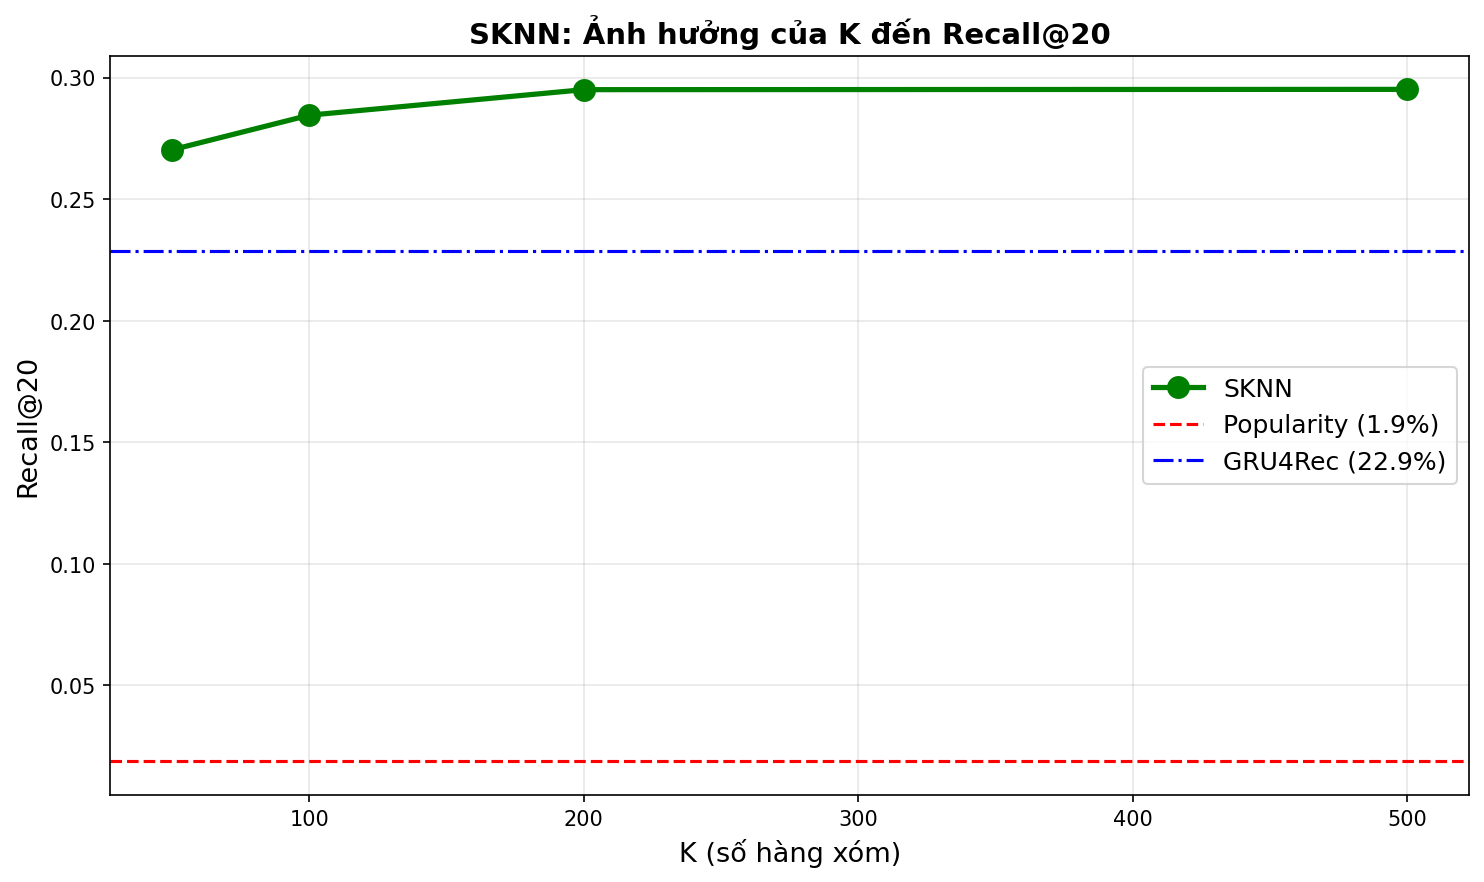
\includegraphics[width=0.75\textwidth]{recall_theo_k_final.png}
\caption{Ảnh hưởng của K đến Recall@20 của SKNN. Nguồn: kết quả thực nghiệm của nhóm từ \texttt{output/all\_results.pkl}, trực quan hóa bằng \texttt{src/plots.py}.}
\label{fig:recall_k}
\end{figure}

\textbf{Nhận xét từ biểu đồ:}
\begin{itemize}
    \item Recall tăng nhanh từ K=50 đến K=200 (giai đoạn ``thiếu hàng xóm'')
    \item Từ K=200 đến K=500, đường cong gần như nằm ngang (0.2951 $\to$ 0.2952) -- đã bão hòa (diminishing returns)
    \item Nếu tiếp tục tăng K (>1000), có thể Recall sẽ giảm do nhiễu từ các phiên kém tương tự
    \item K=200--500 là vùng cân bằng tốt cho dataset này
\end{itemize}

\subsection{Đường cong loss huấn luyện của GRU4Rec}

Hình \ref{fig:loss_curve} thể hiện đường cong loss trong quá trình huấn luyện GRU4Rec qua 10 epoch.

\begin{figure}[H]
\centering
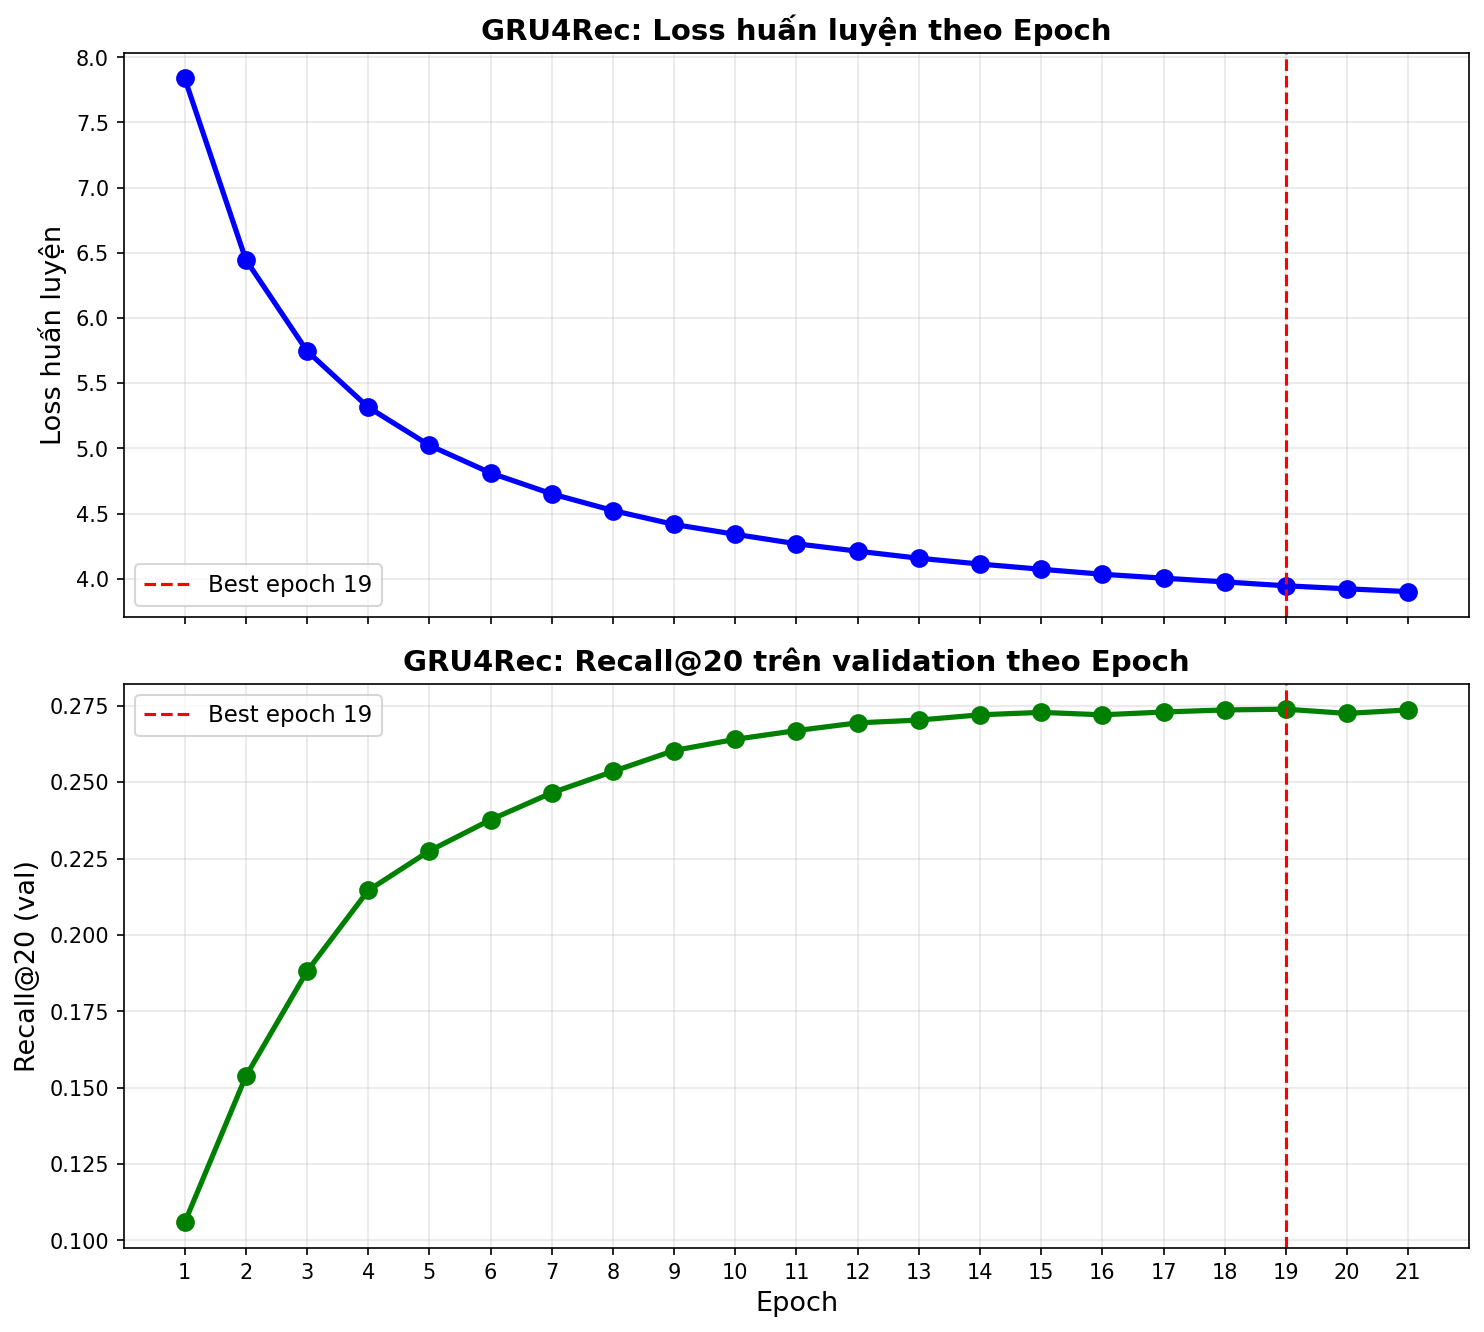
\includegraphics[width=0.75\textwidth]{gru4rec_loss_curve.png}
\caption{Đường cong loss huấn luyện của GRU4Rec qua 10 epoch. Nguồn: kết quả thực nghiệm của nhóm từ \texttt{output/all\_results.pkl}, trực quan hóa bằng \texttt{src/plots.py}.}
\label{fig:loss_curve}
\end{figure}

\textbf{Phân tích đường cong loss:}

\begin{enumerate}
    \item \textbf{Epoch 1--3:} Loss giảm nhanh từ 7.79 (trung bình epoch 1; mức khởi tạo lý thuyết $\ln(10435) \approx 9.25$) xuống 5.69 (epoch 3). Đây là giai đoạn mô hình học được các pattern cơ bản nhất (item phổ biến, co-occurrence đơn giản).

    \item \textbf{Epoch 4--7:} Loss tiếp tục giảm nhưng chậm hơn (từ 5.26 xuống 4.62). Mô hình bắt đầu học các pattern phức tạp hơn (sequential dependencies).

    \item \textbf{Epoch 8--10:} Loss giảm chậm dần (4.51 $\to$ 4.33), chưa hoàn toàn hội tụ -- vẫn còn xu hướng giảm nhẹ.
    
    \item \textbf{Không có overfitting rõ ràng:} Loss không tăng trở lại, cho thấy mô hình chưa overfit trên training set. Có thể huấn luyện thêm epoch để cải thiện.
\end{enumerate}

\textbf{Gợi ý cải thiện:}
\begin{itemize}
    \item Tăng số epoch lên 20--30 để mô hình hội tụ tốt hơn
    \item Sử dụng learning rate scheduling (giảm lr khi loss bão hòa)
    \item Tăng hidden size (256 hoặc 512) để tăng capacity
    \item Thêm early stopping dựa trên validation loss
\end{itemize}

\newpage


% ============================================================
% CHƯƠNG 4: PHÂN TÍCH VÀ THẢO LUẬN
% ============================================================
\section{PHÂN TÍCH VÀ THẢO LUẬN}
\label{chap:analysis}

\subsection{So sánh tổng hợp 3 mô hình}

Bảng \ref{tab:final_comparison} tổng hợp kết quả của cả ba mô hình trên bộ dữ liệu Yoochoose (1/64).

\begin{table}[H]
\centering
\caption{Bảng so sánh tổng hợp kết quả 3 mô hình}
\label{tab:final_comparison}
\begin{tabular}{lccccc}
\toprule
\textbf{Mô hình} & \textbf{Recall@20} & \textbf{MRR@20} & \textbf{$\Delta$Recall} & \textbf{Thời gian} & \textbf{GPU} \\
\midrule
Popularity Baseline & 0.0187 & 0.0041 & -- & $\sim$5s & Không \\
SKNN (K=500) & \textbf{0.2952} & \textbf{0.1349} & +0.2765 & $\sim$2s & Không \\
GRU4Rec (10 epoch) & 0.2796 & 0.1262 & +0.2609 & $\sim$3 phút & Có \\
\bottomrule
\end{tabular}
\end{table}

Hình \ref{fig:comparison} minh họa trực quan sự khác biệt giữa 3 mô hình.

\begin{figure}[H]
\centering
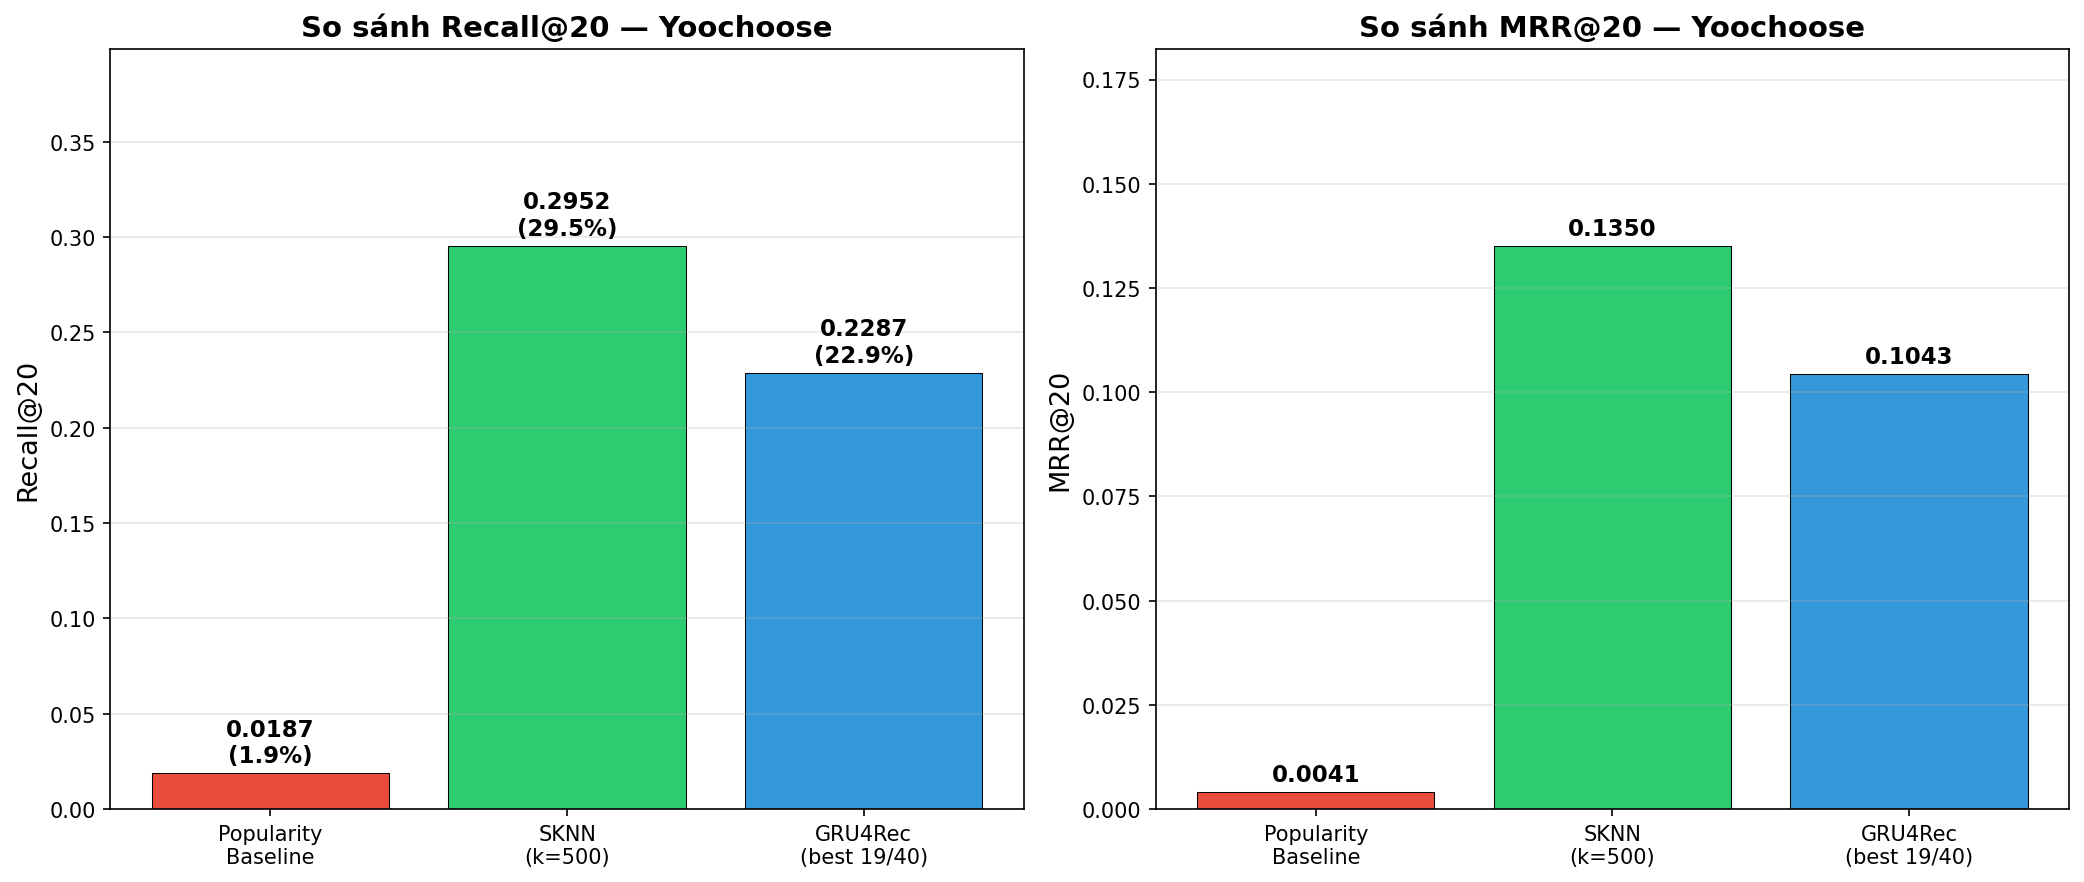
\includegraphics[width=0.85\textwidth]{so_sanh_final.png}
\caption{Biểu đồ so sánh Recall@20 và MRR@20 của 3 mô hình. Nguồn: kết quả thực nghiệm của nhóm từ \texttt{output/all\_results.pkl}, trực quan hóa bằng \texttt{src/plots.py}.}
\label{fig:comparison}
\end{figure}

\textbf{Nhận xét tổng quan:}
\begin{enumerate}
    \item Cả SKNN và GRU4Rec đều cải thiện rõ so với Popularity Baseline (hơn 26 điểm Recall).
    \item SKNN cao hơn GRU4Rec một mức nhỏ (+1.56 điểm Recall, +0.0087 MRR) trên cấu hình thí nghiệm này.
    \item Việc SKNN ngang ngửa hoặc vượt GRU4Rec là kết quả thường gặp, phù hợp với các nghiên cứu trước \cite{ludewig2018, jannach2017}.
\end{enumerate}

\subsection{Phân tích tại sao SKNN vượt Popularity (+27.65 điểm)}

Mức cải thiện của SKNN so với Popularity Baseline (+27.65 điểm Recall, tương đương khoảng $15.8$ lần theo tỉ lệ Recall) có thể được giải thích bởi các yếu tố sau:

\subsubsection{Tận dụng thông tin phiên hiện tại}

Popularity Baseline không sử dụng thông tin từ phiên hiện tại -- nó gợi ý cùng một danh sách item cho mọi người dùng, bất kể họ đang xem gì. Ngược lại, SKNN sử dụng phiên hiện tại để tìm các phiên tương tự, từ đó sinh khuyến nghị \textbf{cá nhân hóa theo ngữ cảnh}.

\textbf{Ví dụ minh họa:}
\begin{itemize}
    \item Phiên hiện tại: [Laptop, Chuột, Bàn phím]
    \item Popularity gợi ý: [iPhone, Áo thun, Giày] (item phổ biến nhất, không liên quan)
    \item SKNN tìm phiên tương tự: [Laptop, Chuột, Bàn phím, \textbf{Tai nghe}]
    \item SKNN gợi ý: [\textbf{Tai nghe}, Webcam, USB Hub] (liên quan đến ngữ cảnh)
\end{itemize}

\subsubsection{Khai thác co-occurrence pattern}

SKNN ngầm khai thác mối quan hệ đồng xuất hiện (co-occurrence) giữa các item. Nếu item A và item B thường xuất hiện cùng nhau trong nhiều session, thì khi phiên hiện tại chứa A, SKNN sẽ có xu hướng gợi ý B (vì nhiều phiên hàng xóm chứa cả A và B).

\subsubsection{Phân tích định lượng}

\begin{table}[H]
\centering
\caption{Phân tích chi tiết sự cải thiện của SKNN so với Popularity}
\label{tab:sknn_vs_pop}
\begin{tabular}{lcc}
\toprule
\textbf{Chỉ số} & \textbf{Popularity} & \textbf{SKNN} \\
\midrule
Recall@20 & 0.0187 & 0.2952 \\
Cải thiện tuyệt đối & -- & +0.2765 \\
Cải thiện tương đối & -- & $\times$15.8 lần \\
\midrule
MRR@20 & 0.0041 & 0.1349 \\
Cải thiện tuyệt đối & -- & +0.1308 \\
Cải thiện tương đối & -- & $\times$32.9 lần \\
\bottomrule
\end{tabular}
\end{table}

MRR cải thiện mạnh hơn Recall ($\times$32.9 vs $\times$15.8), cho thấy SKNN không chỉ tìm đúng item mà còn đặt item đúng ở vị trí cao hơn nhiều trong danh sách.

\subsection{Phân tích tại sao GRU4Rec chưa vượt SKNN}

Trên cấu hình thí nghiệm này, GRU4Rec thấp hơn SKNN 1.56 điểm Recall. Tuy nhiên, về \emph{lý thuyết} GRU4Rec vẫn có những ưu thế quan trọng mà điều kiện thí nghiệm hạn chế (mẫu 1/64, 10 epoch) chưa cho phép phát huy:

\subsubsection{Học được thứ tự (Sequential patterns)}

SKNN coi mỗi session như một \textbf{tập hợp} item (bỏ qua thứ tự). GRU4Rec coi session như một \textbf{chuỗi} có thứ tự và học được rằng:
\begin{itemize}
    \item Chuỗi $[A \rightarrow B \rightarrow C]$ có ý nghĩa khác với $[C \rightarrow B \rightarrow A]$
    \item Item gần đây (cuối chuỗi) có ảnh hưởng lớn hơn item xa (đầu chuỗi)
    \item Có những transition pattern: ``sau khi xem A thường xem B'' mà SKNN không nắm bắt được
\end{itemize}

\subsubsection{Biểu diễn liên tục (Continuous representation)}

GRU4Rec biểu diễn mỗi item bằng vector embedding dense trong không gian liên tục $\mathbb{R}^d$. Điều này cho phép:
\begin{itemize}
    \item Nắm bắt sự tương tự ngữ nghĩa giữa các item (item tương tự có embedding gần nhau)
    \item Tổng quát hóa tốt hơn cho item hiếm (thông qua embedding được chia sẻ)
    \item Mã hóa thông tin phong phú hơn so với biểu diễn nhị phân (có/không) của SKNN
\end{itemize}

\subsubsection{Tại sao GRU4Rec lại thấp hơn SKNN ở đây?}

Có nhiều lý do giải thích tại sao GRU4Rec chưa vượt được SKNN trong thí nghiệm này:

\begin{enumerate}
    \item \textbf{Session ngắn:} Với session trung bình chỉ 3.7 item (trung vị 3), lợi thế ``học thứ tự'' của GRU bị hạn chế. Thứ tự chỉ thực sự quan trọng khi chuỗi đủ dài.

    \item \textbf{Dữ liệu hạn chế:} Chỉ dùng mẫu 1/64 ($\sim$108K phiên train) -- chưa đủ để GRU học tốt embedding cho hơn 10K item. Trên toàn bộ dataset, GRU thường thu hẹp hoặc vượt khoảng cách này.

    \item \textbf{Chưa hội tụ:} GRU4Rec chỉ được huấn luyện 10 epoch, loss vẫn đang giảm (4.41 $\to$ 4.33 ở epoch 9--10), chưa hoàn toàn hội tụ. Với nhiều epoch hơn, kết quả nhiều khả năng cải thiện thêm.

    \item \textbf{SKNN là baseline mạnh:} Như Ludewig \& Jannach (2018) \cite{ludewig2018} đã chỉ ra, các phương pháp neighborhood là mốc so sánh cạnh tranh với nhiều mô hình học sâu, đặc biệt khi item phổ biến lặp lại giữa các phiên gần nhau như trong dữ liệu thương mại điện tử Yoochoose.
\end{enumerate}

\subsection{Ưu nhược điểm từng phương pháp}

\begin{table}[H]
\centering
\caption{Phân tích ưu nhược điểm chi tiết}
\label{tab:pros_cons}
\begin{tabular}{L{2.7cm}L{5.4cm}L{5.4cm}}
\toprule
\textbf{Mô hình} & \textbf{Ưu điểm} & \textbf{Nhược điểm} \\
\midrule
\textbf{Popularity} & 
\begin{itemize}[leftmargin=0.3cm, topsep=0pt]
    \item Đơn giản về mặt triển khai
    \item Không cần tính toán
    \item Baseline tốt để so sánh
    \item Luôn có kết quả (không fail)
\end{itemize} &
\begin{itemize}[leftmargin=0.3cm, topsep=0pt]
    \item Không cá nhân hóa
    \item Bỏ qua ngữ cảnh phiên
    \item Hiệu quả thấp trong cấu hình này
    \item Gợi ý giống nhau cho mọi user
\end{itemize} \\
\midrule
\textbf{SKNN} &
\begin{itemize}[leftmargin=0.3cm, topsep=0pt]
    \item Không cần huấn luyện
    \item Không cần GPU
    \item Dễ triển khai, dễ debug
    \item Giải thích được (interpretable)
    \item Dễ cập nhật (thêm session mới)
    \item Hiệu quả cao
\end{itemize} &
\begin{itemize}[leftmargin=0.3cm, topsep=0pt]
    \item Bỏ qua thứ tự click
    \item Cần lưu toàn bộ session lịch sử
    \item Tốc độ chậm khi N lớn
    \item Không học được biểu diễn item
    \item Khó mở rộng cho dataset rất lớn
\end{itemize} \\
\midrule
\textbf{GRU4Rec} &
\begin{itemize}[leftmargin=0.3cm, topsep=0pt]
    \item Học được thứ tự click
    \item Biểu diễn item liên tục
    \item Inference nhanh (vài ms)
    \item Tổng quát hóa tốt
    \item Có thể mở rộng (scalable)
\end{itemize} &
\begin{itemize}[leftmargin=0.3cm, topsep=0pt]
    \item Cần huấn luyện (tốn thời gian)
    \item Cần GPU cho training
    \item Khó giải thích (black-box)
    \item Nhiều hyperparameter cần tune
    \item Khó cập nhật incremental
    \item Cần nhiều dữ liệu để học tốt
\end{itemize} \\
\bottomrule
\end{tabular}
\end{table}

\subsection{Ảnh hưởng của siêu tham số K}

Phân tích chi tiết hơn về ảnh hưởng của K trong SKNN:

\subsubsection{Cơ chế ảnh hưởng}

Hyperparameter $K$ kiểm soát \textbf{trade-off giữa precision và coverage}:

\begin{itemize}
    \item \textbf{K nhỏ (precision cao, coverage thấp):} Chỉ xét ít phiên rất tương tự $\rightarrow$ item được gợi ý có độ tin cậy cao nhưng đa dạng thấp. Có thể bỏ sót item tốt từ phiên ít tương tự hơn.
    
    \item \textbf{K lớn (precision thấp hơn, coverage cao):} Xét nhiều phiên, kể cả phiên ít tương tự $\rightarrow$ danh sách gợi ý đa dạng hơn nhưng dễ chịu ảnh hưởng từ các phiên ít liên quan.
\end{itemize}

\subsubsection{Phân tích theo lý thuyết bias--variance}

\begin{itemize}
    \item \textbf{K nhỏ $\rightarrow$ High variance:} Kết quả phụ thuộc nhiều vào vài phiên cụ thể. Nếu phiên hàng xóm ``may mắn'' chứa item đúng $\rightarrow$ hit. Nếu không $\rightarrow$ miss.
    
    \item \textbf{K lớn $\rightarrow$ High bias:} Kết quả bị ``trung bình hóa'' bởi nhiều phiên, có xu hướng ưu tiên item phổ biến và giảm mức cá nhân hóa theo phiên truy vấn.
    
    \item \textbf{K đạt kết quả cao nhất trong dải thử nghiệm:} Cân bằng giữa bias và variance. Trong thí nghiệm, K=500 cho Recall@20 cao nhất trên dataset này.
\end{itemize}

\subsubsection{Khuyến nghị chọn K trong thực tế}

\begin{enumerate}
    \item Bắt đầu với K=100--500 (phạm vi thường cho kết quả tốt)
    \item Dùng validation set để tune K
    \item Xem xét trade-off giữa chất lượng và tốc độ
    \item K phù hợp phụ thuộc vào đặc điểm dataset (kích thước, sparsity, diversity)
\end{enumerate}

\subsection{Hạn chế của thí nghiệm}

Các kết quả trên nên được đọc trong phạm vi thiết kế thí nghiệm, thay vì xem như kết luận tuyệt đối cho mọi hệ thống khuyến nghị:

\begin{enumerate}
    \item \textbf{Mẫu dữ liệu 1/64:} Cách lấy mẫu giúp thí nghiệm phù hợp với tài nguyên tính toán hiện có, nhưng số liệu tuyệt đối có thể thay đổi khi dùng toàn bộ Yoochoose. Kết luận đáng tin hơn ở đây là thứ tự tương đối trong cùng cấu hình: Popularity thấp rõ rệt, GRU4Rec và SKNN cao hơn rõ.

    \item \textbf{Một miền dữ liệu:} Yoochoose là clickstream thương mại điện tử. Kết quả chưa tự động suy rộng sang tin tức, nhạc, giáo dục, hoặc dataset tiếng Việt nếu hành vi phiên khác đáng kể.

    \item \textbf{GRU4Rec mới được huấn luyện ở mức vừa phải:} Mô hình chạy 10 epoch và chưa tune rộng learning rate, dropout, batch size hay loss. Vì vậy việc GRU4Rec thấp hơn SKNN trong thí nghiệm này không phủ định tiềm năng của mô hình tuần tự sâu; nó chỉ phản ánh cấu hình đang xét.

    \item \textbf{Chưa thử các biến thể mạnh hơn:} Phần thực nghiệm chưa bao gồm V-SKNN, STAN, NARM, SR-GNN, hoặc GRU4Rec với BPR loss. Các biến thể này có thể thay đổi thứ hạng mô hình.

    \item \textbf{Đánh giá offline:} Recall@20 và MRR@20 đo khả năng dự đoán item cuối trong tập test cố định. Chúng chưa thay thế được A/B testing, nơi các yếu tố như tỷ lệ click, chuyển đổi và trải nghiệm người dùng mới được quan sát trực tiếp.

    \item \textbf{Chỉ dùng chuỗi click:} Thí nghiệm chưa dùng category, price, thời điểm truy cập, dwell time hoặc thông tin nội dung item. Đây là những tín hiệu có thể giúp mô hình phân biệt ý định phiên tốt hơn.

    \item \textbf{Giao thức leave-one-out còn hẹp:} Mỗi phiên test chỉ dùng item cuối làm nhãn. Một hệ thống thực tế có thể cần đánh giá ở nhiều vị trí trong phiên hoặc đo chất lượng của cả danh sách gợi ý theo thời gian.
\end{enumerate}

\newpage


% ============================================================
% CHƯƠNG 5: KẾT LUẬN VÀ HƯỚNG PHÁT TRIỂN
% ============================================================
\section{KẾT LUẬN VÀ HƯỚNG PHÁT TRIỂN}
\label{chap:conclusion}

\subsection{Tóm tắt kết quả}

Báo cáo này trình bày bài toán Session-based Recommendation trong bối cảnh người dùng ẩn danh, nơi hệ thống phải dự đoán item tiếp theo chỉ từ chuỗi click ngắn của phiên hiện tại.

\textbf{Các kết quả chính:}

\begin{enumerate}
    \item \textbf{Popularity Baseline} (Recall@20 = 1.87\%): Kết quả này cho thấy việc chỉ gợi ý item phổ biến không đủ cho bài toán theo phiên, nhưng vẫn cần giữ làm mốc so sánh tối thiểu.

    \item \textbf{SKNN với K=500} (Recall@20 = 29.52\%, MRR@20 = 0.1349): Phương pháp dựa trên phiên lân cận đạt kết quả cao nhất trong thí nghiệm, cao hơn Popularity +27.65 điểm Recall@20. Điểm mạnh của SKNN là không cần huấn luyện và có thể diễn giải qua các phiên hàng xóm.

    \item \textbf{GRU4Rec với 10 epoch} (Recall@20 = 27.96\%, MRR@20 = 0.1262): Mô hình học sâu đạt kết quả gần SKNN nhưng \textbf{chưa vượt} (thấp hơn 1.56 điểm Recall) trong cấu hình mẫu 1/64 và 10 epoch. Kết quả này hợp lý vì GRU4Rec thường cần nhiều dữ liệu, nhiều epoch và tune siêu tham số kỹ hơn.
\end{enumerate}

\textbf{Kết luận quan trọng:}
\begin{itemize}
    \item Thông tin trong phiên hiện tại, dù chỉ gồm vài click, đã cải thiện chất lượng gợi ý đáng kể so với popularity thuần túy.
    \item SKNN là baseline mạnh và dễ giải thích; vì vậy nên xem nó là mốc so sánh nghiêm túc trước khi kết luận một mô hình học sâu là tốt hơn.
    \item GRU4Rec có lợi thế khi học thứ tự click, nhưng \textbf{không mặc định vượt SKNN} nếu dữ liệu ít, phiên ngắn hoặc quá trình huấn luyện chưa được tối ưu.
\end{itemize}

\subsection{Đóng góp chính}

Về mặt học thuật và triển khai, bài làm có các đóng góp sau:

\begin{enumerate}
    \item \textbf{Trình bày lý thuyết có kiểm chứng:} Diễn giải SKNN và GRU4Rec từ công thức, trực giác, mã giả đến độ phức tạp, giúp người đọc theo dõi được vì sao thuật toán sinh ra danh sách gợi ý.

    \item \textbf{Triển khai thực nghiệm tái lập:} Pipeline xử lý dữ liệu, huấn luyện, đánh giá và vẽ biểu đồ được tách thành package \texttt{src/}; notebook chỉ dùng để trình bày và gọi lại logic đã kiểm thử.

    \item \textbf{So sánh cùng điều kiện:} Ba mô hình được đánh giá trên cùng tập train/test, cùng protocol leave-one-out và cùng hai metric Recall@20, MRR@20.

    \item \textbf{Phân tích ảnh hưởng của K:} Thí nghiệm với nhiều giá trị K cho thấy chất lượng SKNN tăng rồi bão hòa, từ đó giải thích vì sao chọn K=500 trong cấu hình cuối.

    \item \textbf{Diễn giải kết quả không thổi phồng:} Báo cáo nêu rõ SKNN thắng trong cấu hình hiện tại, đồng thời chỉ ra những điều kiện mà GRU4Rec có thể được cải thiện thêm.
\end{enumerate}

\subsection{Hướng mở rộng}

Nếu tiếp tục phát triển đề tài, các hướng sau là hợp lý nhất vì bám trực tiếp vào hạn chế đã nêu:

\subsubsection{NARM -- Neural Attentive Recommendation Machine}

NARM (Li et al., 2017) \cite{li2017} mở rộng GRU4Rec bằng cách thêm cơ chế Attention:

\begin{equation}
    \alpha_t = \text{softmax}(q^T \sigma(W_1 h_t + W_2 h_T))
\end{equation}
\begin{equation}
    c = \sum_{t=1}^{T} \alpha_t h_t
\end{equation}

Attention cho phép mô hình ``chú ý'' đến những bước thời gian quan trọng nhất, thay vì chỉ dựa vào hidden state cuối cùng. Điều này đặc biệt hữu ích khi session dài và có nhiều item không liên quan (noise).

\textbf{Ưu điểm so với GRU4Rec:}
\begin{itemize}
    \item Nắm bắt được cả local preference (item gần đây) và global preference (toàn bộ session)
    \item Giải thích được phần nào (attention weights cho biết item nào quan trọng)
    \item Có thể cải thiện so với GRU4Rec trong các thiết lập được báo cáo bởi Li et al. \cite{li2017}
\end{itemize}

\subsubsection{SR-GNN -- Session-based Recommendation with Graph Neural Networks}

SR-GNN (Wu et al., 2019) \cite{wu2019} mô hình hóa session dưới dạng đồ thị có hướng:

\begin{itemize}
    \item Mỗi item là một node
    \item Mỗi transition (click từ item A sang item B) là một edge
    \item Sử dụng Graph Neural Network để học biểu diễn item trong đồ thị phiên
\end{itemize}

\textbf{Ưu điểm:}
\begin{itemize}
    \item Nắm bắt được quan hệ phức tạp giữa các item (không chỉ sequential)
    \item Xử lý tốt trường hợp item lặp lại trong session
    \item Đạt kết quả cạnh tranh trên nhiều benchmark được báo cáo trong bài gốc \cite{wu2019}
\end{itemize}

\subsubsection{BERT4Rec -- Bidirectional Encoder Representations for Recommendation}

BERT4Rec áp dụng kiến trúc Transformer (self-attention) cho recommendation \cite{sun2019, vaswani2017}:

\begin{itemize}
    \item Sử dụng masked item prediction (tương tự masked language model trong NLP)
    \item Bidirectional: xem xét cả context trái và phải
    \item Multi-head self-attention cho phép nắm bắt nhiều loại quan hệ
\end{itemize}

\textbf{Ưu điểm:}
\begin{itemize}
    \item Không bị giới hạn bởi vanishing gradient (không dùng RNN)
    \item Parallel computation (nhanh hơn RNN khi training)
    \item Nắm bắt long-range dependencies tốt hơn
\end{itemize}

\subsubsection{Dataset tiếng Việt}

Một hướng mở rộng thực tế và có giá trị cao là thu thập và thí nghiệm trên dataset từ các nền tảng thương mại điện tử Việt Nam:

\begin{itemize}
    \item \textbf{Tiki:} Nền tảng e-commerce lớn tại Việt Nam
    \item \textbf{Shopee Vietnam:} Marketplace phổ biến nhất
    \item \textbf{Sendo:} Nền tảng nội địa
    \item \textbf{VnExpress:} Trang tin tức (session-based article recommendation)
\end{itemize}

Dataset tiếng Việt sẽ giúp:
\begin{enumerate}
    \item Đánh giá hiệu quả các phương pháp trên hành vi người dùng Việt Nam
    \item Khám phá đặc thù riêng (ví dụ: ảnh hưởng của ngày lễ, flash sale)
    \item Đóng góp cho cộng đồng nghiên cứu trong nước
\end{enumerate}

\subsubsection{Các hướng khác}

\begin{table}[H]
\centering
\caption{Tổng hợp các hướng mở rộng}
\label{tab:future_work}
\begin{tabular}{llc}
\toprule
\textbf{Hướng} & \textbf{Mô tả} & \textbf{Độ khó} \\
\midrule
NARM & Thêm Attention vào GRU & $\star\star\star$ \\
SR-GNN & Session dạng đồ thị + GNN & $\star\star\star\star$ \\
BERT4Rec & Transformer bidirectional & $\star\star\star\star$ \\
SASRec & Self-Attention Sequential & $\star\star\star\star$ \\
Dataset Việt Nam & Thu thập từ Tiki/Shopee & $\star\star\star$ \\
Context-aware & Thêm time, category, price & $\star\star$ \\
Cross-session & Liên kết nhiều session cùng user & $\star\star\star$ \\
Real-time serving & Deploy model lên production & $\star\star\star\star$ \\
\bottomrule
\end{tabular}
\end{table}

\newpage


% ============================================================
% TÀI LIỆU THAM KHẢO
% ============================================================
\newpage
\renewcommand{\refname}{TÀI LIỆU THAM KHẢO}
\begin{thebibliography}{99}

\bibitem{hidasi2016}
Hidasi, B., Karatzoglou, A., Baltrunas, L., \& Tikk, D. (2016).
\textit{Session-based Recommendations with Recurrent Neural Networks}.
In Proceedings of the International Conference on Learning Representations (ICLR 2016).
arXiv:1511.06939. \url{https://arxiv.org/abs/1511.06939}

\bibitem{ludewig2018}
Ludewig, M., \& Jannach, D. (2018).
\textit{Evaluation of Session-based Recommendation Algorithms}.
User Modeling and User-Adapted Interaction (UMUAI), 28(4-5), 331--390.
arXiv:1803.09587. \url{https://arxiv.org/abs/1803.09587}

\bibitem{jannach2017}
Jannach, D., Ludewig, M., \& Lerche, L. (2017).
\textit{When Recurrent Neural Networks meet the Neighborhood for Session-Based Recommendation}.
In Proceedings of the 11th ACM Conference on Recommender Systems (RecSys 2017), pp. 306--310. DOI: 10.1145/3109859.3109872. \url{https://doi.org/10.1145/3109859.3109872}

\bibitem{li2017}
Li, J., Ren, P., Chen, Z., Ren, Z., Lian, T., \& Ma, J. (2017).
\textit{Neural Attentive Session-based Recommendation}.
In Proceedings of the 2017 ACM Conference on Information and Knowledge Management (CIKM 2017), pp. 1419--1428. DOI: 10.1145/3038912.3052569. arXiv:1711.04725. \url{https://arxiv.org/abs/1711.04725}

\bibitem{cho2014}
Cho, K., van Merriënboer, B., Gulcehre, C., Bahdanau, D., Bougares, F., Schwenk, H., \& Bengio, Y. (2014).
\textit{Learning Phrase Representations using RNN Encoder-Decoder for Statistical Machine Translation}.
In Proceedings of the 2014 Conference on Empirical Methods in Natural Language Processing (EMNLP 2014), pp. 1724--1734. arXiv:1406.1078. \url{https://arxiv.org/abs/1406.1078}

\bibitem{rendle2009}
Rendle, S., Freudenthaler, C., Gantner, Z., \& Schmidt-Thieme, L. (2009).
\textit{BPR: Bayesian Personalized Ranking from Implicit Feedback}.
In Proceedings of the 25th Conference on Uncertainty in Artificial Intelligence (UAI 2009), pp. 452--461. arXiv:1205.2618. \url{https://arxiv.org/abs/1205.2618}

\bibitem{wu2019}
Wu, S., Tang, Y., Zhu, Y., Wang, L., Xie, X., \& Tan, T. (2019).
\textit{Session-based Recommendation with Graph Neural Networks}.
In Proceedings of the AAAI Conference on Artificial Intelligence (AAAI 2019), 33(01), 346--353. arXiv:1811.00855. \url{https://arxiv.org/abs/1811.00855}

\bibitem{goodfellow2016}
Goodfellow, I., Bengio, Y., \& Courville, A. (2016).
\textit{Deep Learning}.
MIT Press. \url{https://www.deeplearningbook.org/}

\bibitem{koren2009}
Koren, Y., Bell, R., \& Volinsky, C. (2009).
\textit{Matrix Factorization Techniques for Recommender Systems}.
Computer, 42(8), 30--37. DOI: 10.1109/MC.2009.263. \url{https://doi.org/10.1109/MC.2009.263}

\bibitem{sarwar2001}
Sarwar, B., Karypis, G., Konstan, J., \& Riedl, J. (2001).
\textit{Item-based Collaborative Filtering Recommendation Algorithms}.
In Proceedings of the 10th International Conference on World Wide Web (WWW 2001), pp. 285--295. DOI: 10.1145/371920.372071. \url{https://files.grouplens.org/papers/www10_sarwar.pdf}

\bibitem{hochreiter1997}
Hochreiter, S., \& Schmidhuber, J. (1997).
\textit{Long Short-Term Memory}.
Neural Computation, 9(8), 1735--1780. DOI: 10.1162/neco.1997.9.8.1735. \url{https://www.bioinf.jku.at/publications/older/2604.pdf}

\bibitem{vaswani2017}
Vaswani, A., Shazeer, N., Parmar, N., Uszkoreit, J., Jones, L., Gomez, A. N., Kaiser, Ł., \& Polosukhin, I. (2017).
\textit{Attention Is All You Need}.
In Advances in Neural Information Processing Systems (NeurIPS 2017), pp. 5998--6008. arXiv:1706.03762. \url{https://arxiv.org/abs/1706.03762}

\bibitem{sun2019}
Sun, F., Liu, J., Wu, J., Pei, C., Lin, X., Ou, W., \& Jiang, P. (2019).
\textit{BERT4Rec: Sequential Recommendation with Bidirectional Encoder Representations from Transformer}.
arXiv:1904.06690. \url{https://arxiv.org/abs/1904.06690}

\bibitem{yoochoose2015}
YOOCHOOSE GmbH. (2015).
\textit{RecSys Challenge 2015 Dataset}.
Kaggle dataset mirror. \url{https://www.kaggle.com/datasets/chadgostopp/recsys-challenge-2015}

\end{thebibliography}

\newpage


% ============================================================
% PHỤ LỤC
% ============================================================
\appendix
\setcounter{table}{0}
\setcounter{lstlisting}{0}
\renewcommand{\thetable}{P.\arabic{table}}
\renewcommand{\thelstlisting}{P.\arabic{lstlisting}}
\lstset{basicstyle=\ttfamily\footnotesize}
\phantomsection
\section*{PHỤ LỤC}
\addcontentsline{toc}{section}{PHỤ LỤC}

Phụ lục chỉ giữ các thông tin cần thiết để tái lập thí nghiệm và đối chiếu phần cài đặt cốt lõi. Mã nguồn đầy đủ nằm trong thư mục \texttt{src/} của dự án.

\phantomsection
\subsection*{A. Hướng dẫn chạy lại thí nghiệm}
\addcontentsline{toc}{subsection}{A. Hướng dẫn chạy lại thí nghiệm}

\textbf{Chuẩn bị môi trường và thư viện:}

\begin{lstlisting}[language=bash, caption={Các lệnh chuẩn bị môi trường}]
python -m venv venv
venv\Scripts\activate
pip install -r requirements.txt
\end{lstlisting}

\textbf{Tải dữ liệu:}
\begin{itemize}[topsep=0pt]
    \item Truy cập nguồn dataset: \href{https://www.kaggle.com/datasets/chadgostopp/recsys-challenge-2015}{Kaggle -- RecSys Challenge 2015}.
    \item Tải \texttt{yoochoose-clicks.dat} và đặt vào thư mục \texttt{data/}.
\end{itemize}

\textbf{Chạy pipeline:}

\begin{lstlisting}[language=bash, caption={Các lệnh chạy thí nghiệm và vẽ biểu đồ}]
python run_all.py
python plot_final.py
\end{lstlisting}

\begin{table}[H]
\centering
\caption{Các tệp quan trọng để tái lập kết quả}
\label{tab:appendix_files}
\begin{tabularx}{\textwidth}{@{}lX@{}}
\toprule
\textbf{Đường dẫn} & \textbf{Vai trò} \\
\midrule
\texttt{src/config.py} & Lưu siêu tham số, seed, đường dẫn dữ liệu và đường dẫn kết quả. \\
\texttt{src/data.py} & Tiền xử lý Yoochoose, chia train/test theo thời gian, lọc item hiếm chỉ trên train. \\
\texttt{src/models/sknn.py} & Cài đặt SKNN bằng chỉ mục đảo. \\
\texttt{src/models/gru4rec.py} & Cài đặt GRU4Rec bằng PyTorch. \\
\texttt{src/evaluate.py} & Tính Recall@20 và MRR@20 theo leave-one-out. \\
\texttt{output/all\_results.pkl} & File kết quả cuối cùng, dùng để vẽ biểu đồ và ghi bảng trong báo cáo. \\
\bottomrule
\end{tabularx}
\end{table}

\phantomsection
\subsection*{B. Trích đoạn cốt lõi của SKNN}
\addcontentsline{toc}{subsection}{B. Trích đoạn cốt lõi của SKNN}

Trích đoạn dưới đây thể hiện hai ý chính của SKNN: xây dựng chỉ mục đảo \texttt{item -> session} và chỉ tính similarity trên những phiên có item trùng với phiên truy vấn.

\begin{lstlisting}[caption={Trích đoạn SKNN với chỉ mục đảo (src/models/sknn.py)}, label={lst:sknn_core}]
class SKNN:
    def __init__(self, k=500):
        self.k = k
        self.train_sets = {}
        self.item2sids = defaultdict(list)

    def fit(self, sessions):
        self.train_sets = {
            sid: set(items) for sid, items in sessions.items()
        }
        for sid, items in self.train_sets.items():
            for item in items:
                self.item2sids[item].append(sid)

    def predict(self, query_session, top_n=20):
        query_set = set(query_session)
        candidates = set()
        for item in query_set:
            candidates.update(self.item2sids.get(item, ()))

        sims = []
        for sid in candidates:
            hist_set = self.train_sets[sid]
            inter = len(query_set & hist_set)
            if inter:
                sim = inter / math.sqrt(len(query_set) * len(hist_set))
                sims.append((sid, sim))

        sims.sort(key=lambda x: x[1], reverse=True)
        scores = defaultdict(float)
        for sid, sim in sims[:self.k]:
            for item in self.train_sets[sid]:
                if item not in query_set:
                    scores[item] += sim

        return sorted(
            scores.items(), key=lambda x: x[1], reverse=True
        )[:top_n]
\end{lstlisting}

\phantomsection
\subsection*{C. Trích đoạn cốt lõi của GRU4Rec và đánh giá}
\addcontentsline{toc}{subsection}{C. Trích đoạn cốt lõi của GRU4Rec và đánh giá}

GRU4Rec mã hóa chuỗi item thành embedding, đưa qua GRU, lấy hidden state cuối cùng rồi sinh score cho toàn bộ item trong từ vựng train.

\begin{lstlisting}[caption={Trích đoạn forward của GRU4Rec (src/models/gru4rec.py)}, label={lst:gru4rec_core}]
class GRU4Rec(nn.Module):
    def __init__(self, n_items, emb_size=64, hidden_size=128,
                 n_layers=1, dropout=0.25):
        super().__init__()
        self.hidden_size = hidden_size
        self.embedding = nn.Embedding(n_items, emb_size, padding_idx=0)
        self.gru = nn.GRU(
            emb_size, hidden_size, num_layers=n_layers,
            batch_first=True, dropout=dropout if n_layers > 1 else 0
        )
        self.dropout = nn.Dropout(dropout)
        self.fc_out = nn.Linear(hidden_size, n_items)

    def forward(self, seq):
        emb = self.dropout(self.embedding(seq))
        lengths = (seq != 0).sum(dim=1).cpu()
        packed = nn.utils.rnn.pack_padded_sequence(
            emb, lengths, batch_first=True, enforce_sorted=False
        )
        gru_out, _ = self.gru(packed)
        gru_out, _ = nn.utils.rnn.pad_packed_sequence(
            gru_out, batch_first=True
        )
        idx = (lengths - 1).unsqueeze(1).unsqueeze(2)
        idx = idx.expand(-1, 1, self.hidden_size).to(gru_out.device)
        h_last = gru_out.gather(1, idx).squeeze(1)
        return self.fc_out(self.dropout(h_last))
\end{lstlisting}

\begin{lstlisting}[caption={Trích đoạn đánh giá leave-one-out}, label={lst:evaluate_core}]
def evaluate_gru(model, test_sessions, item2idx,
                 top_n=20, device='cpu'):
    model.eval()
    hits, mrr_sum, n_eval = 0, 0.0, 0

    with torch.no_grad():
        for items in test_sessions.values():
            input_seq = items[:-1]
            label_idx = item2idx.get(items[-1], 0)
            if label_idx == 0:
                continue

            seq_idx = [item2idx.get(i, 0) for i in input_seq]
            seq_t = torch.LongTensor([seq_idx]).to(device)
            logits = model(seq_t).squeeze(0)

            logits[0] = -float('inf')
            for seen in seq_idx:
                if seen > 0:
                    logits[seen] = -float('inf')

            top_indices = logits.topk(top_n).indices.tolist()
            if label_idx in top_indices:
                hits += 1
                rank = top_indices.index(label_idx) + 1
                mrr_sum += 1.0 / rank
            n_eval += 1

    return hits / n_eval, mrr_sum / n_eval
\end{lstlisting}

% ============================================================
% KẾT THÚC TÀI LIỆU
% ============================================================
\end{document}
